% !TEX root = ../main.tex
\section{实验\chinese{section}}
\subsection{实验题目}
综合实验
\subsection{实验目的}
基于本实验室使用的开发板,综合应用《单片机应用技术》课程所学知识,自行设计一个综合实验,具体内容不限,要求尽可能多的应用MSP430F6638单片机的片内资源和开发板资源。
\subsection{实验仪器和设备}
计算机、开发板、示波器、信号源、电源、Code Composer Studio v5、串口调试助手等。
\subsection{实验步骤}
\begin{lstlisting}[language=C]
/****************************************
  |    P4.3|--> LED_Red
  |    P4.2|--> LED_Green
--|RST P4.1|--> LED_Yellow
****************************************/
\end{lstlisting}
\par\indent 设计一款可以点歌、弹奏的随声听。
\par\indent 要求实现以下功能:
\begin{enumerate}
	\item TFT显示屏作为用户交互界面,主菜单包括点歌、弹奏、查看软件信息3个选项;
	\item 3个LED灯显示当前所处的界面;
	\item 矩阵键盘输入,上方数码管显示矩阵键盘输入的历史记录;
	\item 2个独立按钮作为随机切歌和音量开关;
\end{enumerate}
\subsection{程序清单}
\begin{figure}[htbp]
	\centering
	\caption{项目浏览器}
	\label{MusicPlayer}
	\includegraphics[width=15cm]{bitmap/png/MusicPlayer.png}
\end{figure}
\lstinputlisting{src/code/main.c}
\subsection{实验结果记录与分析}
我拍了视频,但pdf文件不方便展示。如有需要可以联系我,我的邮箱是\href{mailto:Wuzy01@qq.com}{Wuzy01@qq.com}。
\begin{figure}[htbp]
	\centering
	\begin{minipage}[htbp]{7.5cm}
		\centering
		\caption{软件启动,进入主界面}
		\label{MusicPlayer1}
		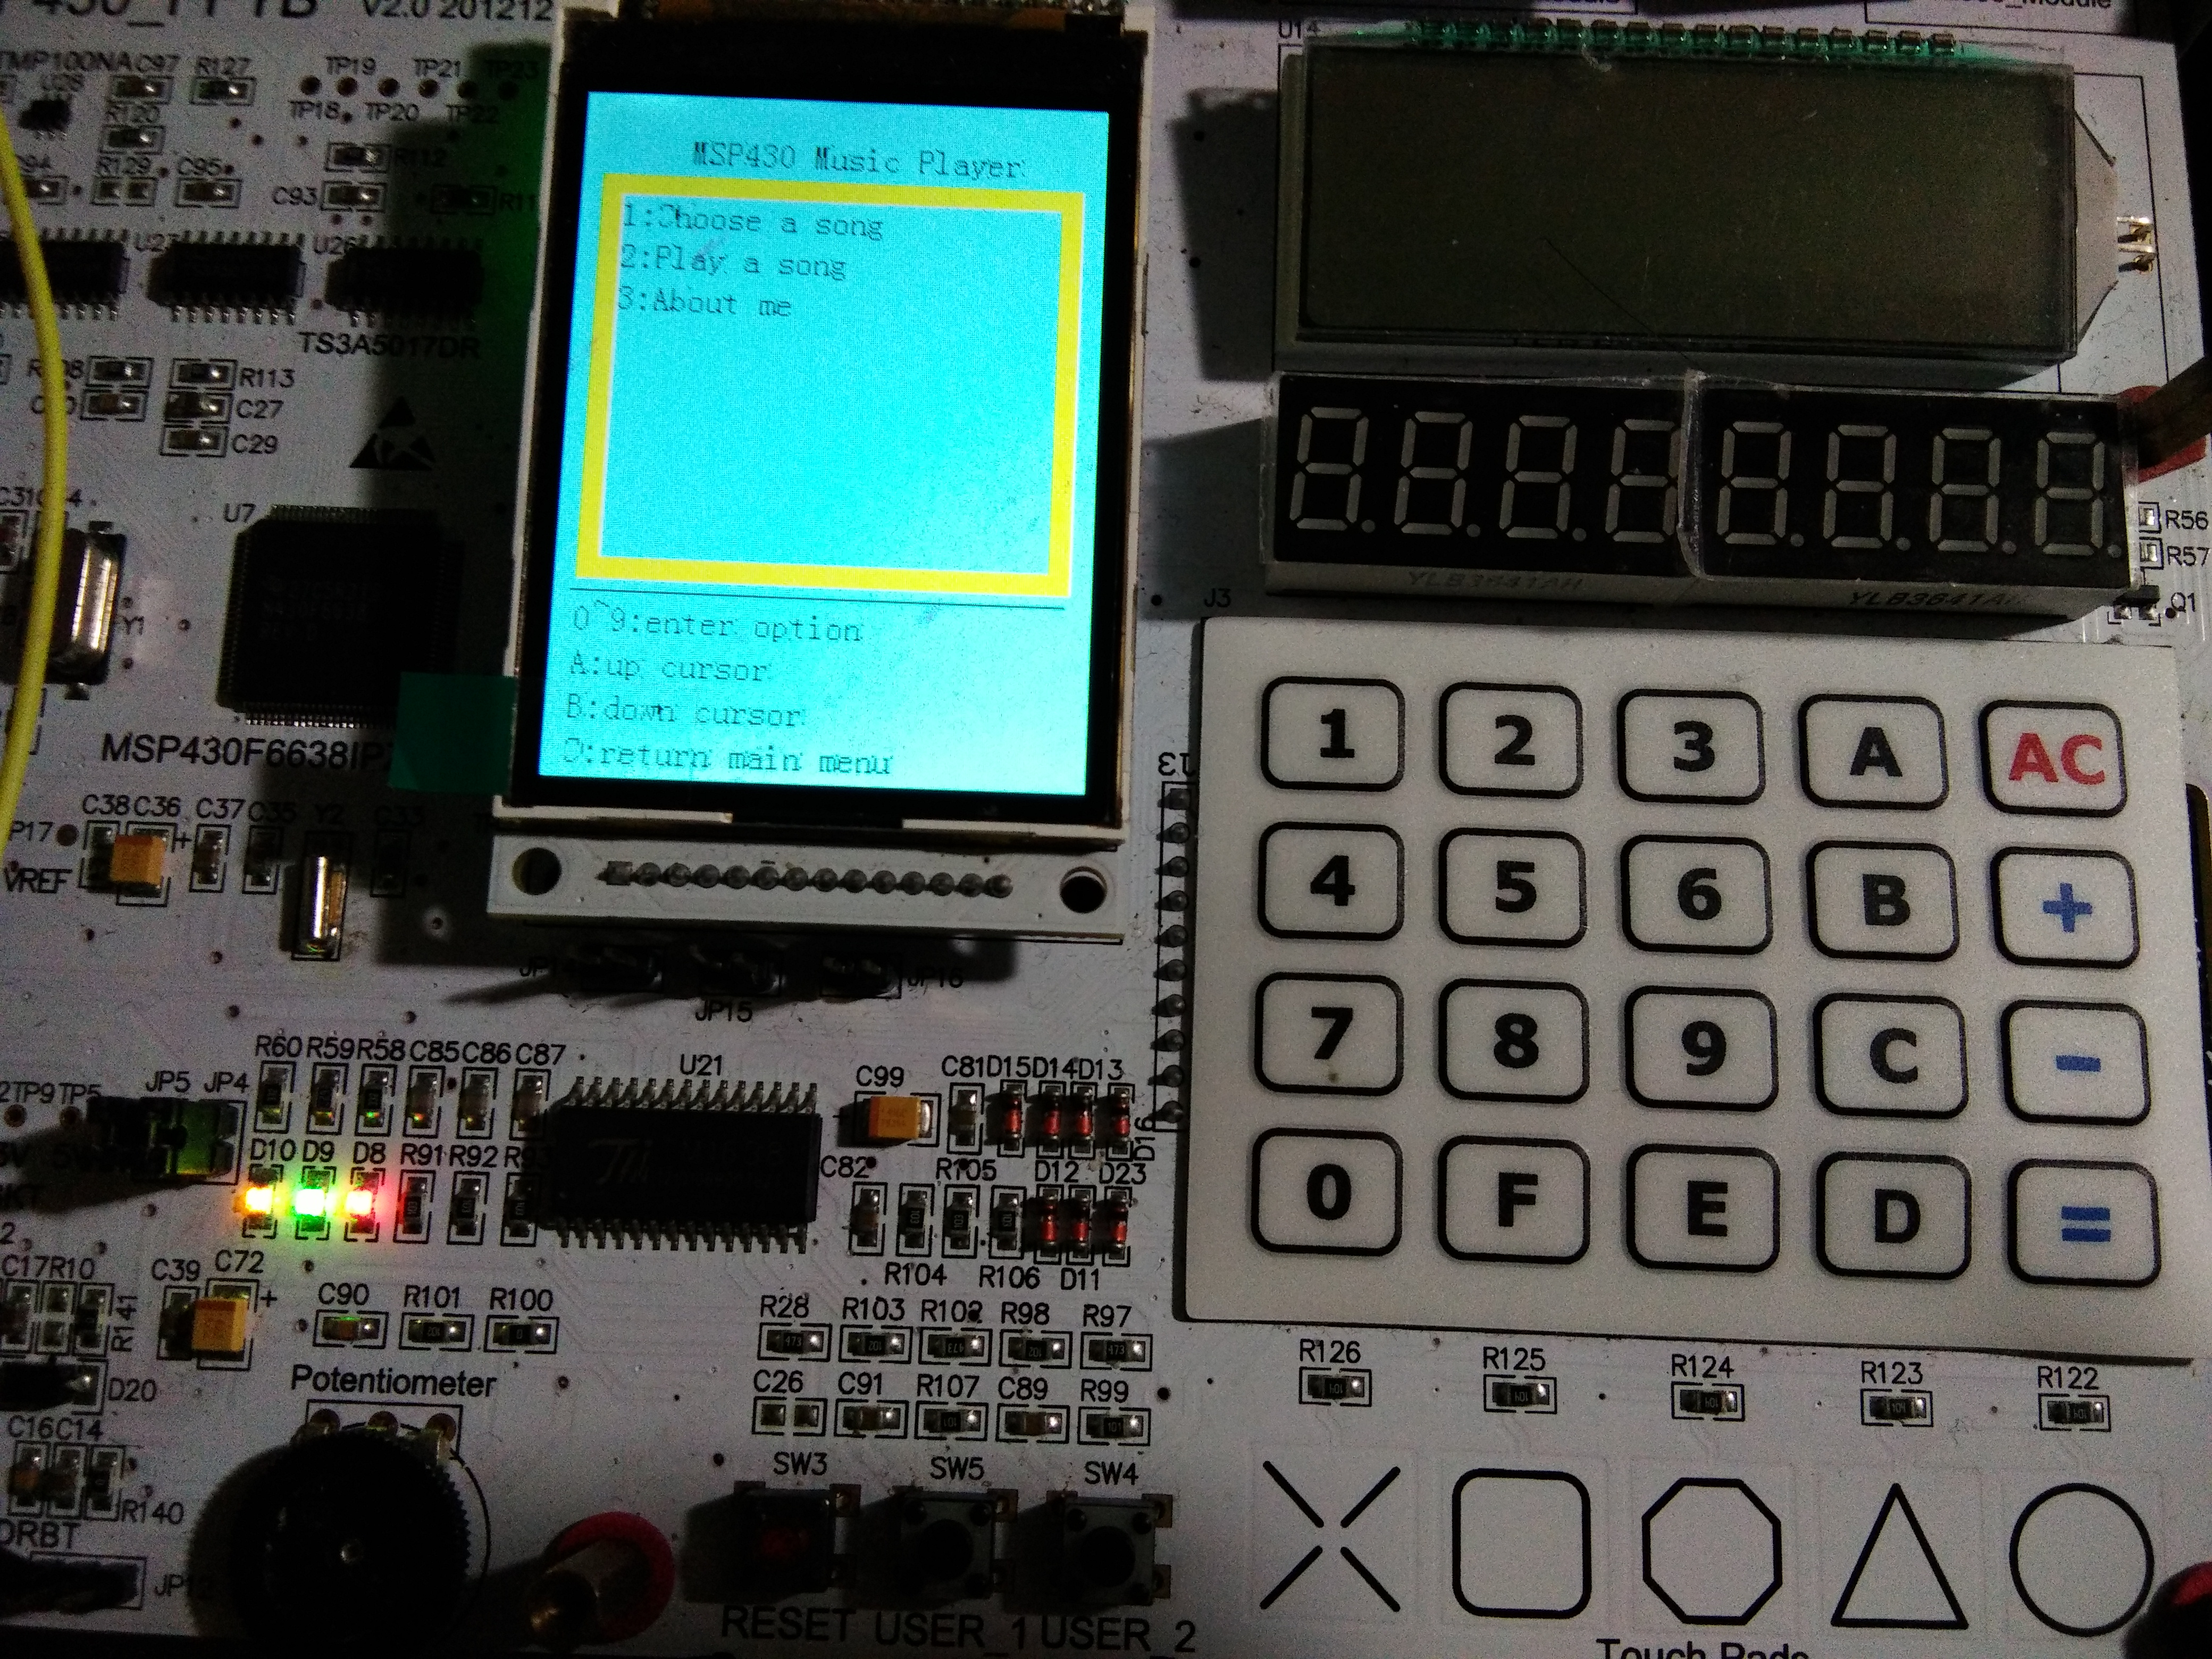
\includegraphics[width=7.5cm]{bitmap/jpg/MusicPlayer1.jpg}
	\end{minipage}
	\begin{minipage}[htbp]{7.5cm}
		\centering
		\caption{按1进入点歌界面}
		\label{MusicPlayer2}
		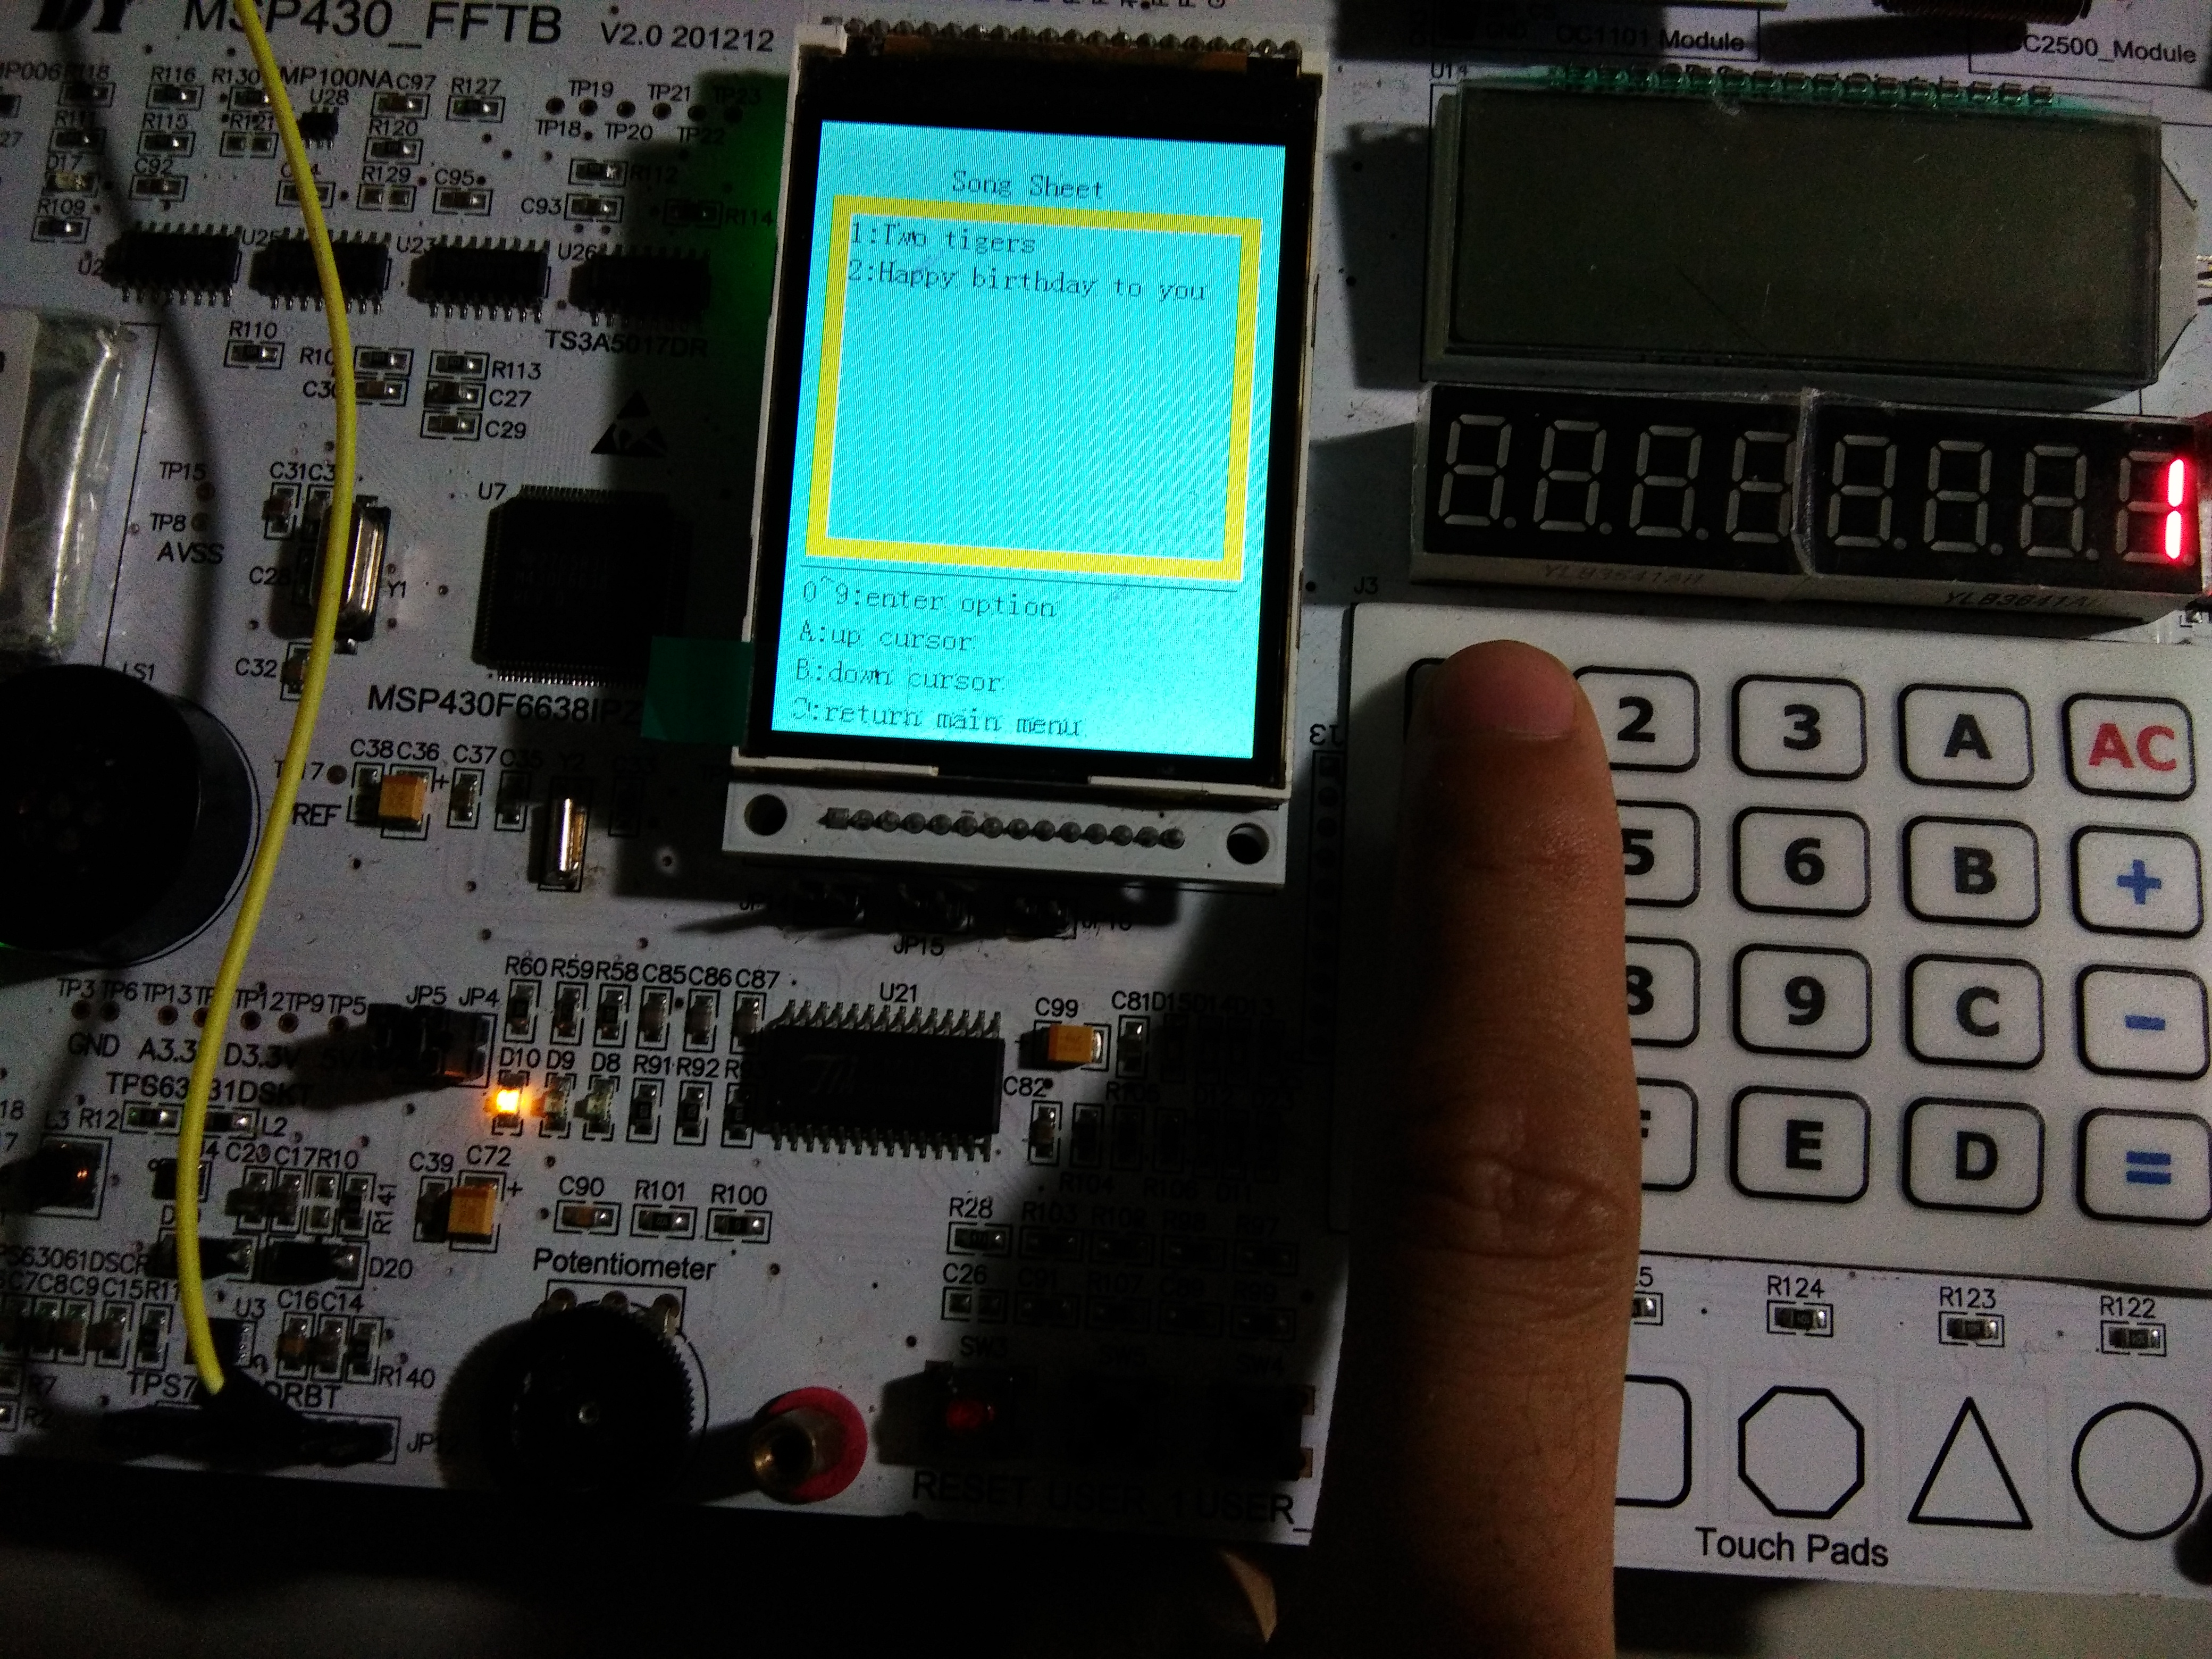
\includegraphics[width=7.5cm]{bitmap/jpg/MusicPlayer2.jpg}
	\end{minipage}
	\begin{minipage}[htbp]{7.5cm}
		\centering
		\caption{按1放第1首歌}
		\label{MusicPlayer3}
		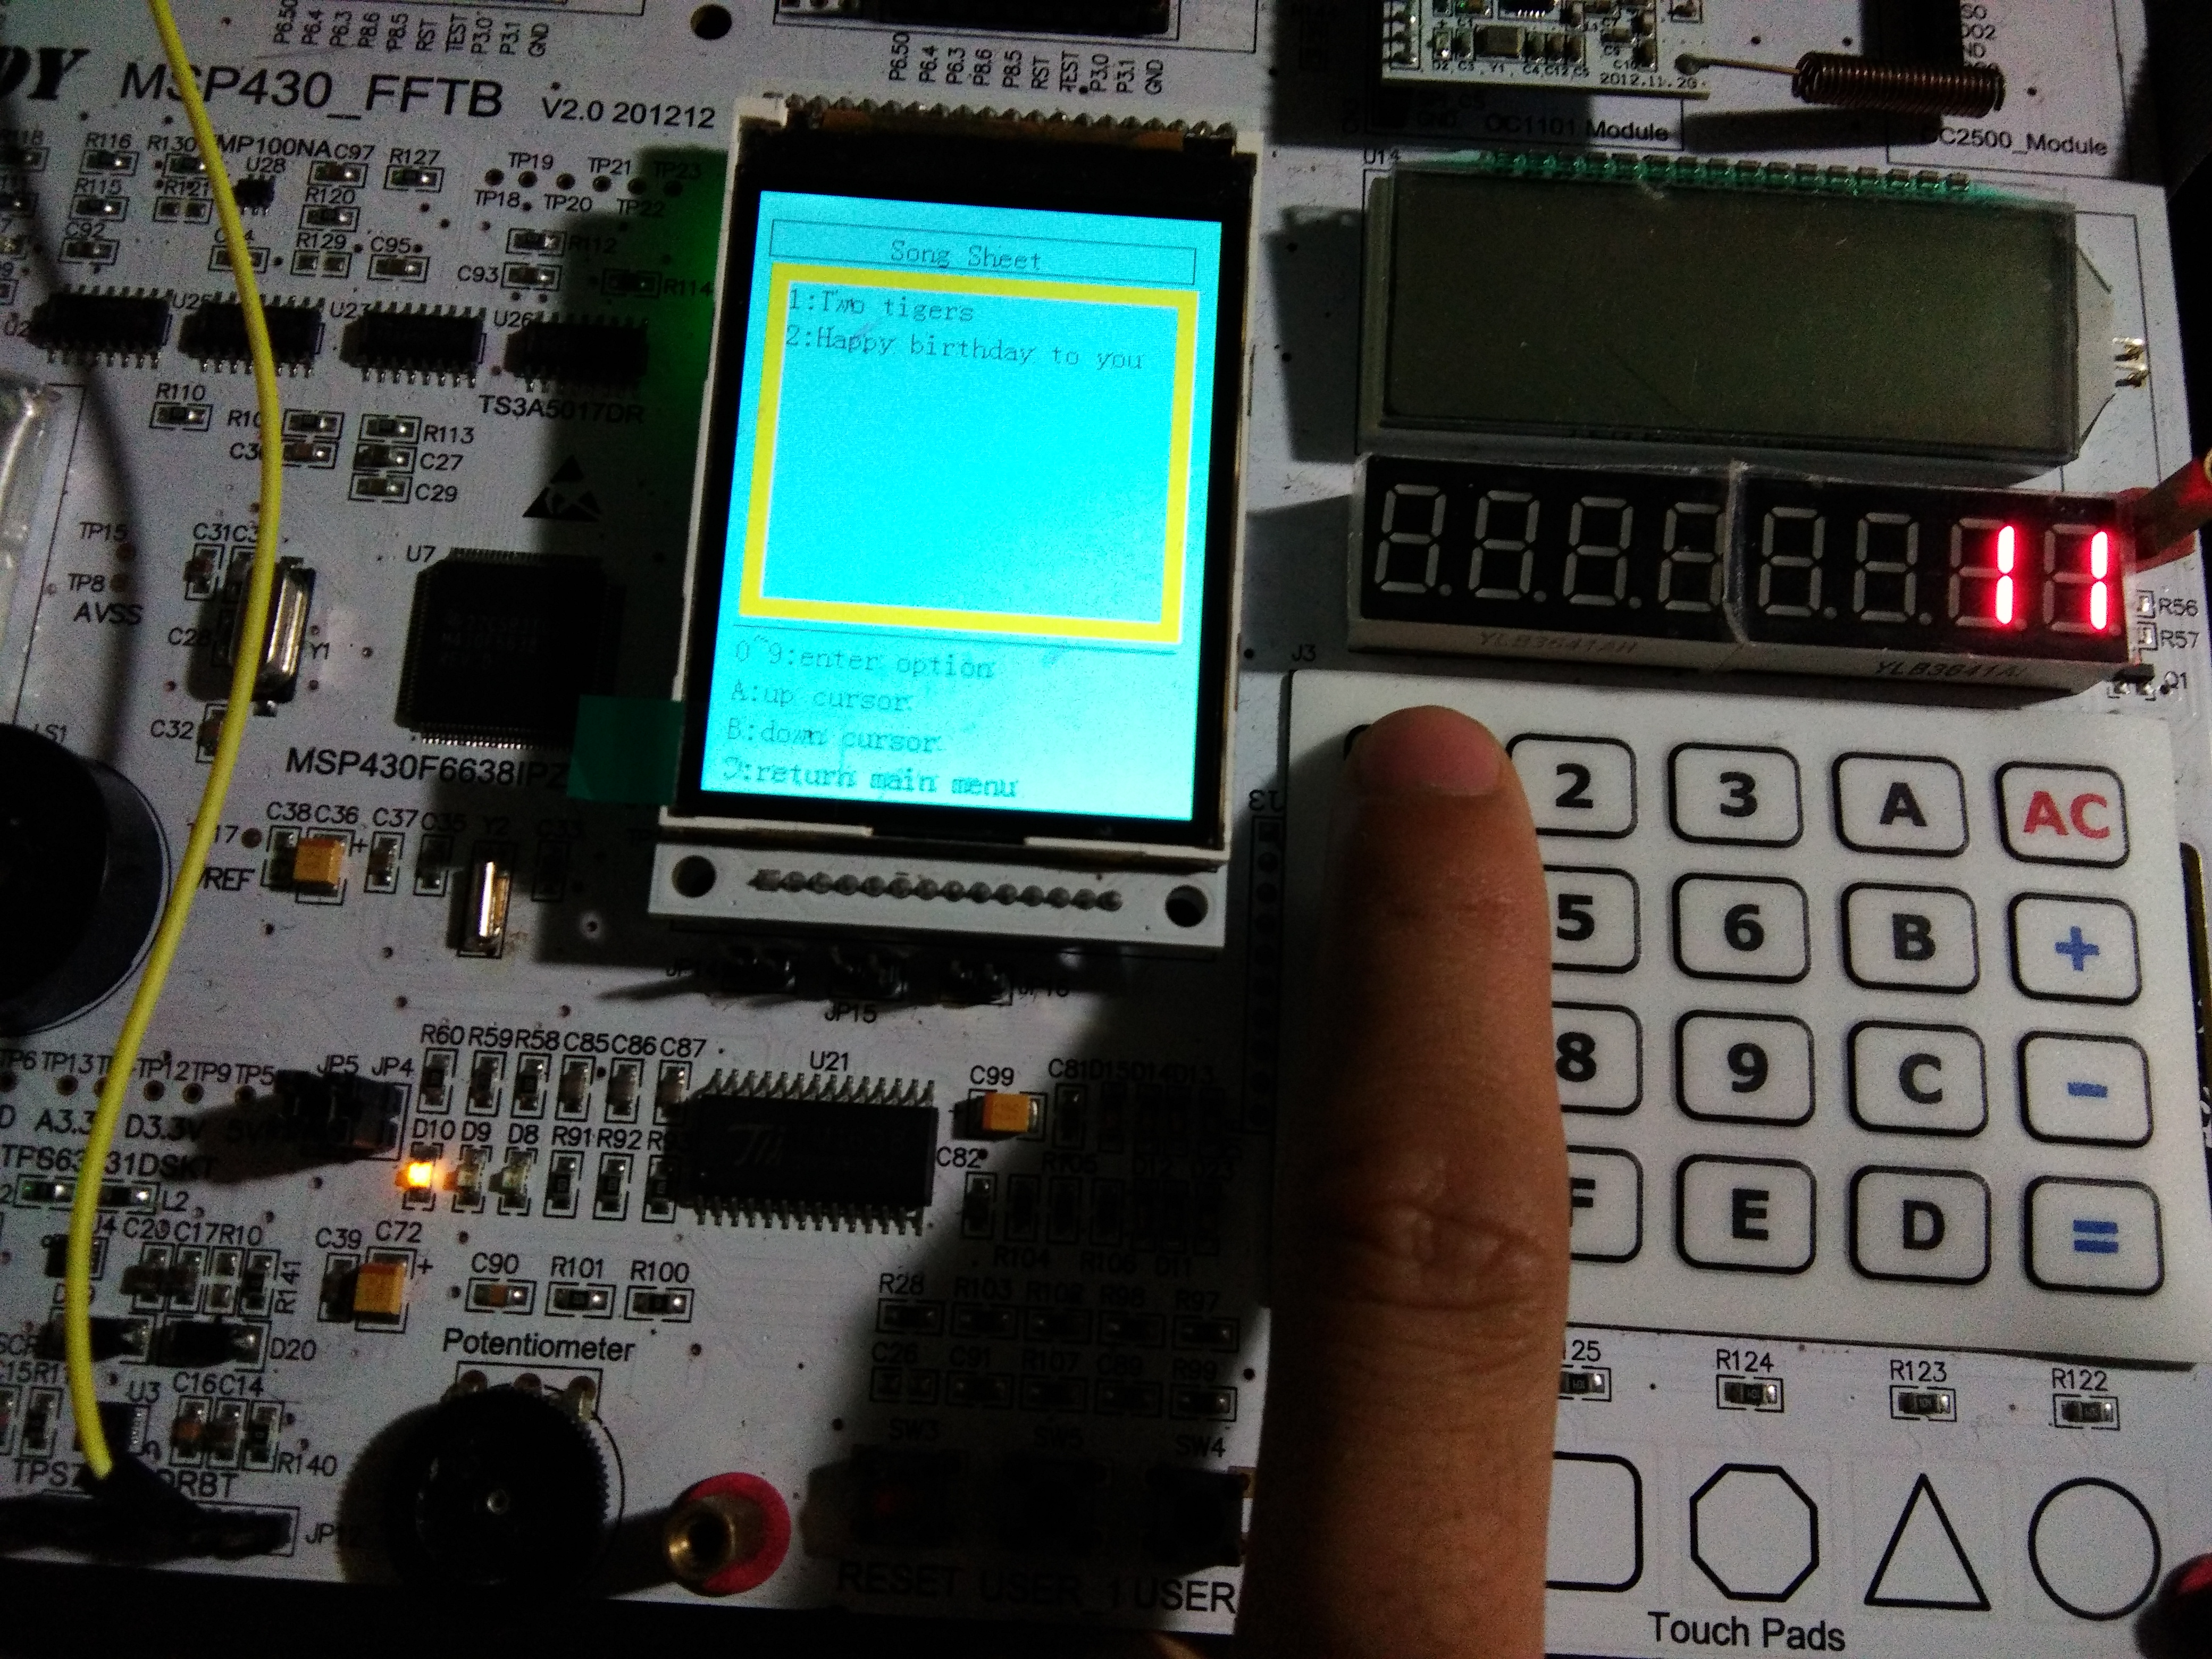
\includegraphics[width=7.5cm]{bitmap/jpg/MusicPlayer3.jpg}
	\end{minipage}
	\begin{minipage}[htbp]{7.5cm}
		\centering
		\caption{按2放第2首歌}
		\label{MusicPlayer4}
		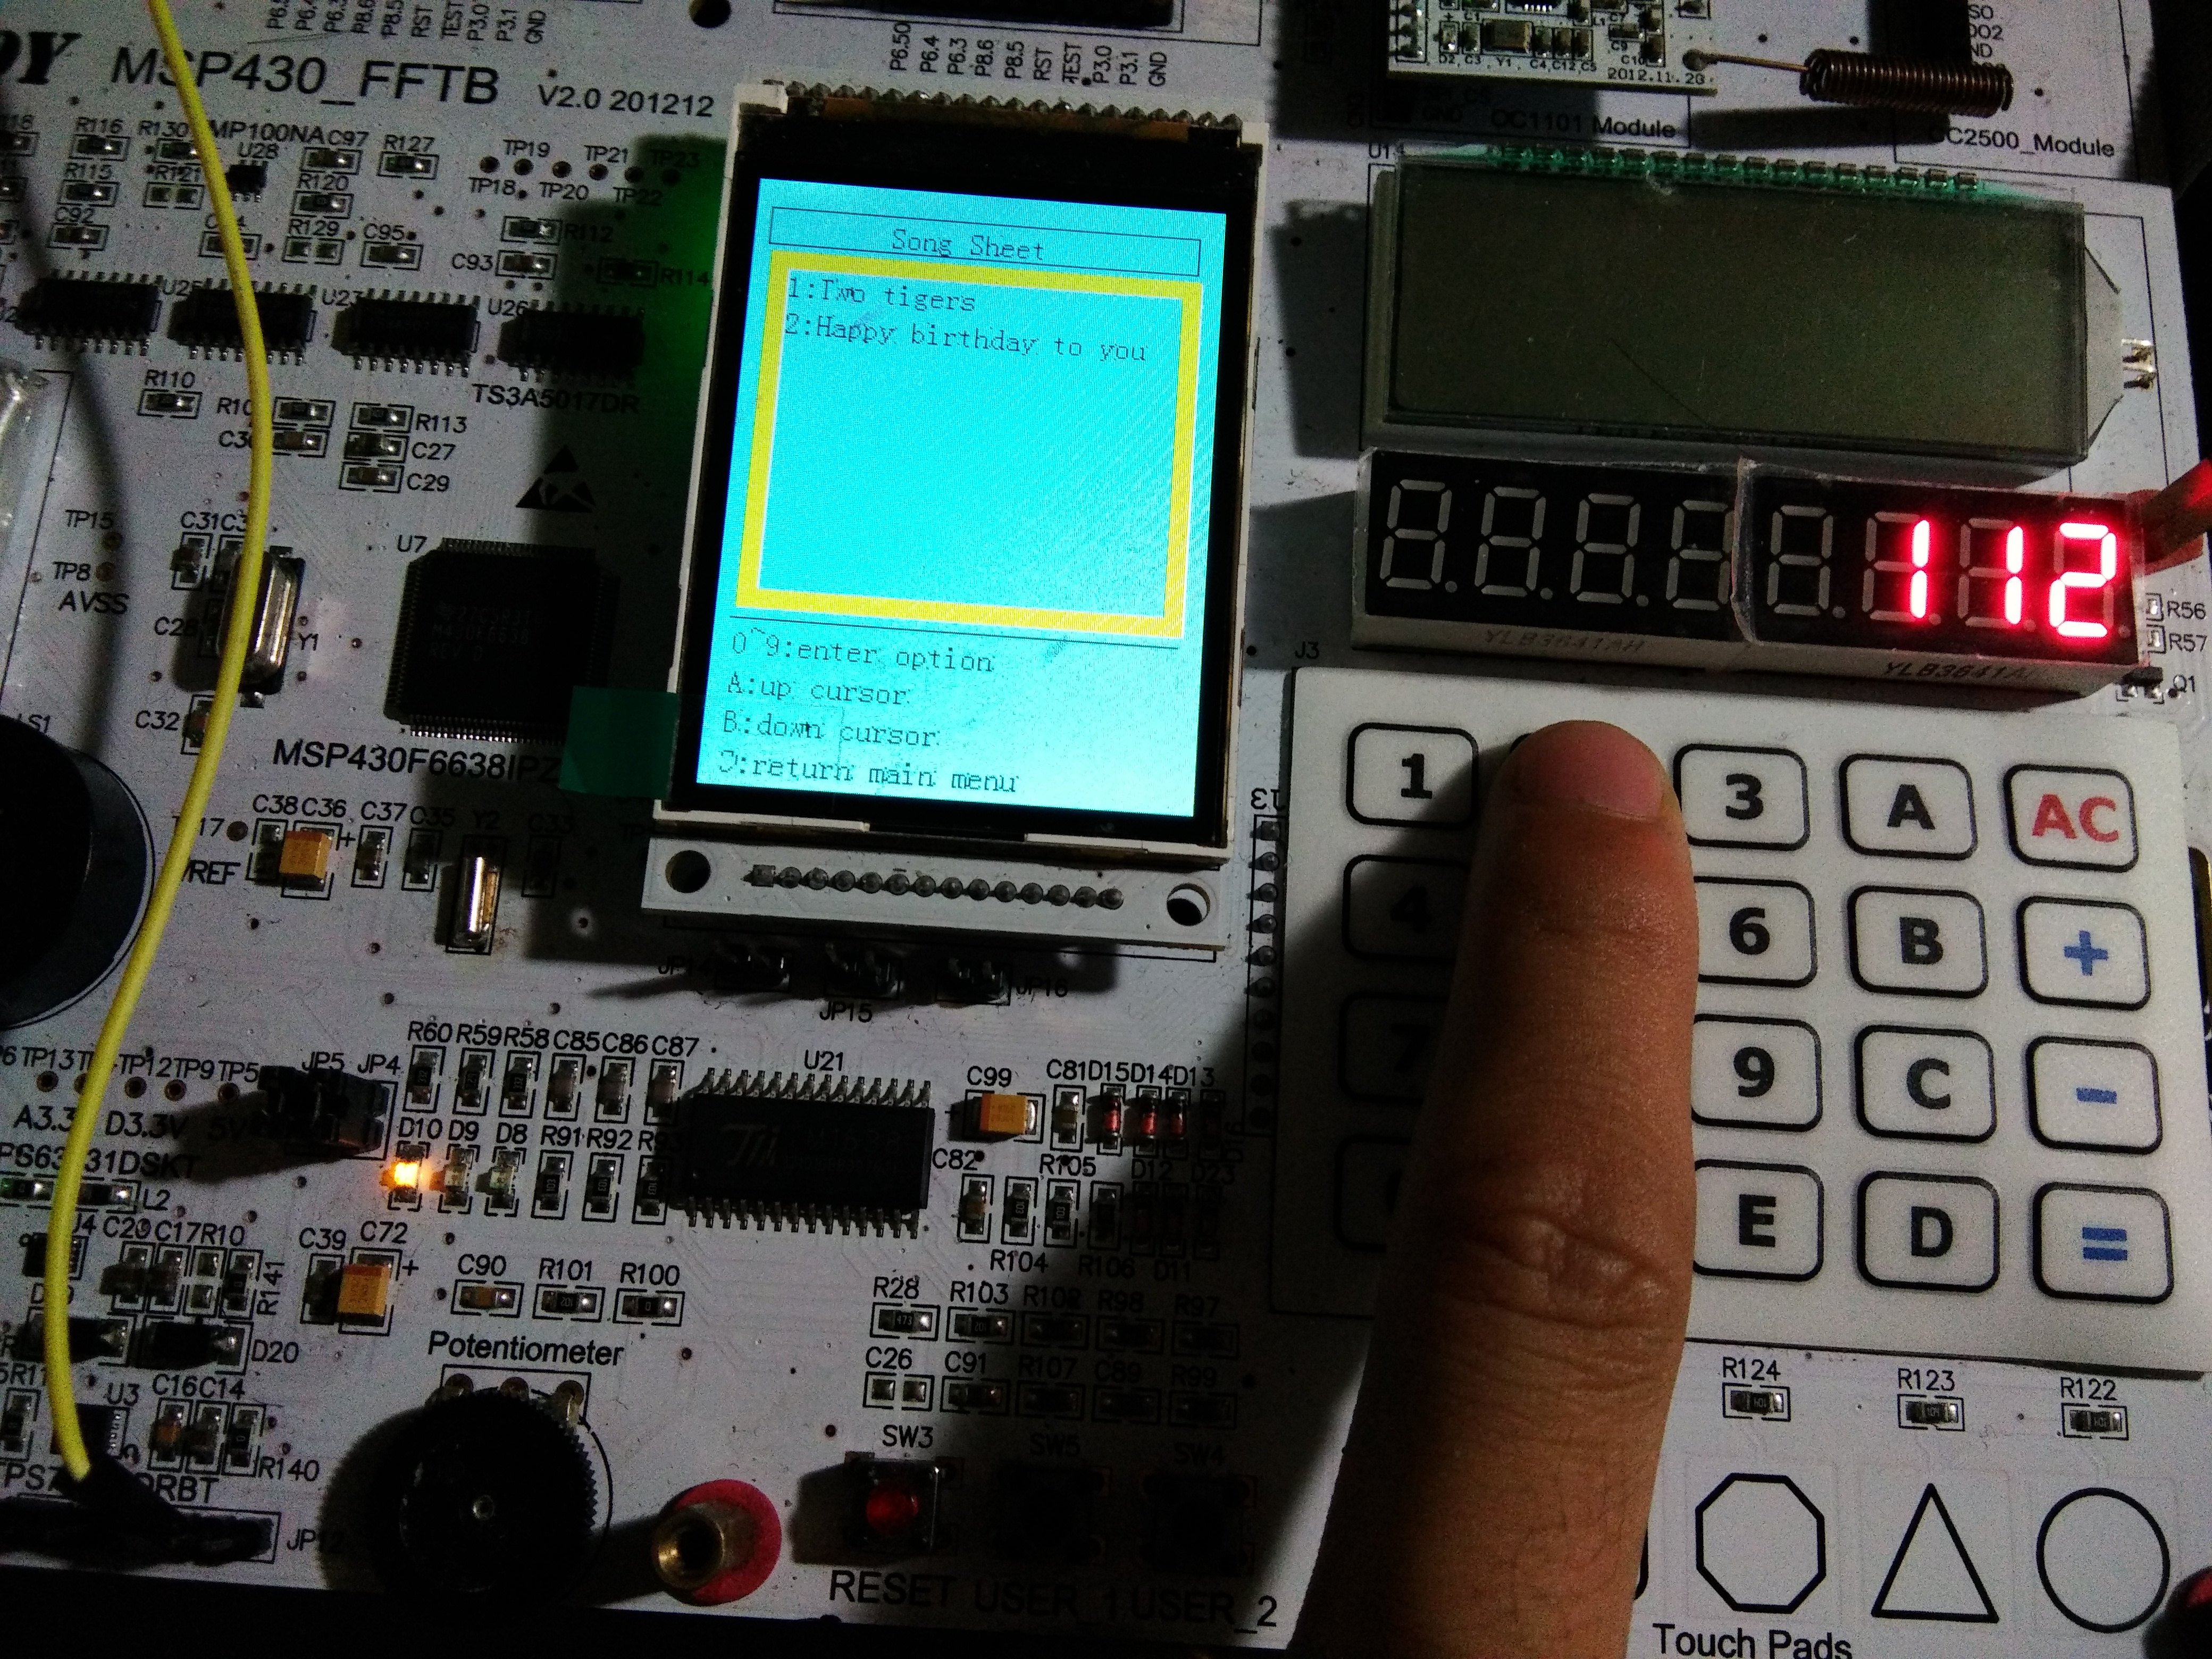
\includegraphics[width=7.5cm]{bitmap/jpg/MusicPlayer4.jpg}
	\end{minipage}
	\begin{minipage}[htbp]{7.5cm}
		\centering
		\caption{按User\_1随机切换歌曲}
		\label{MusicPlayer5}
		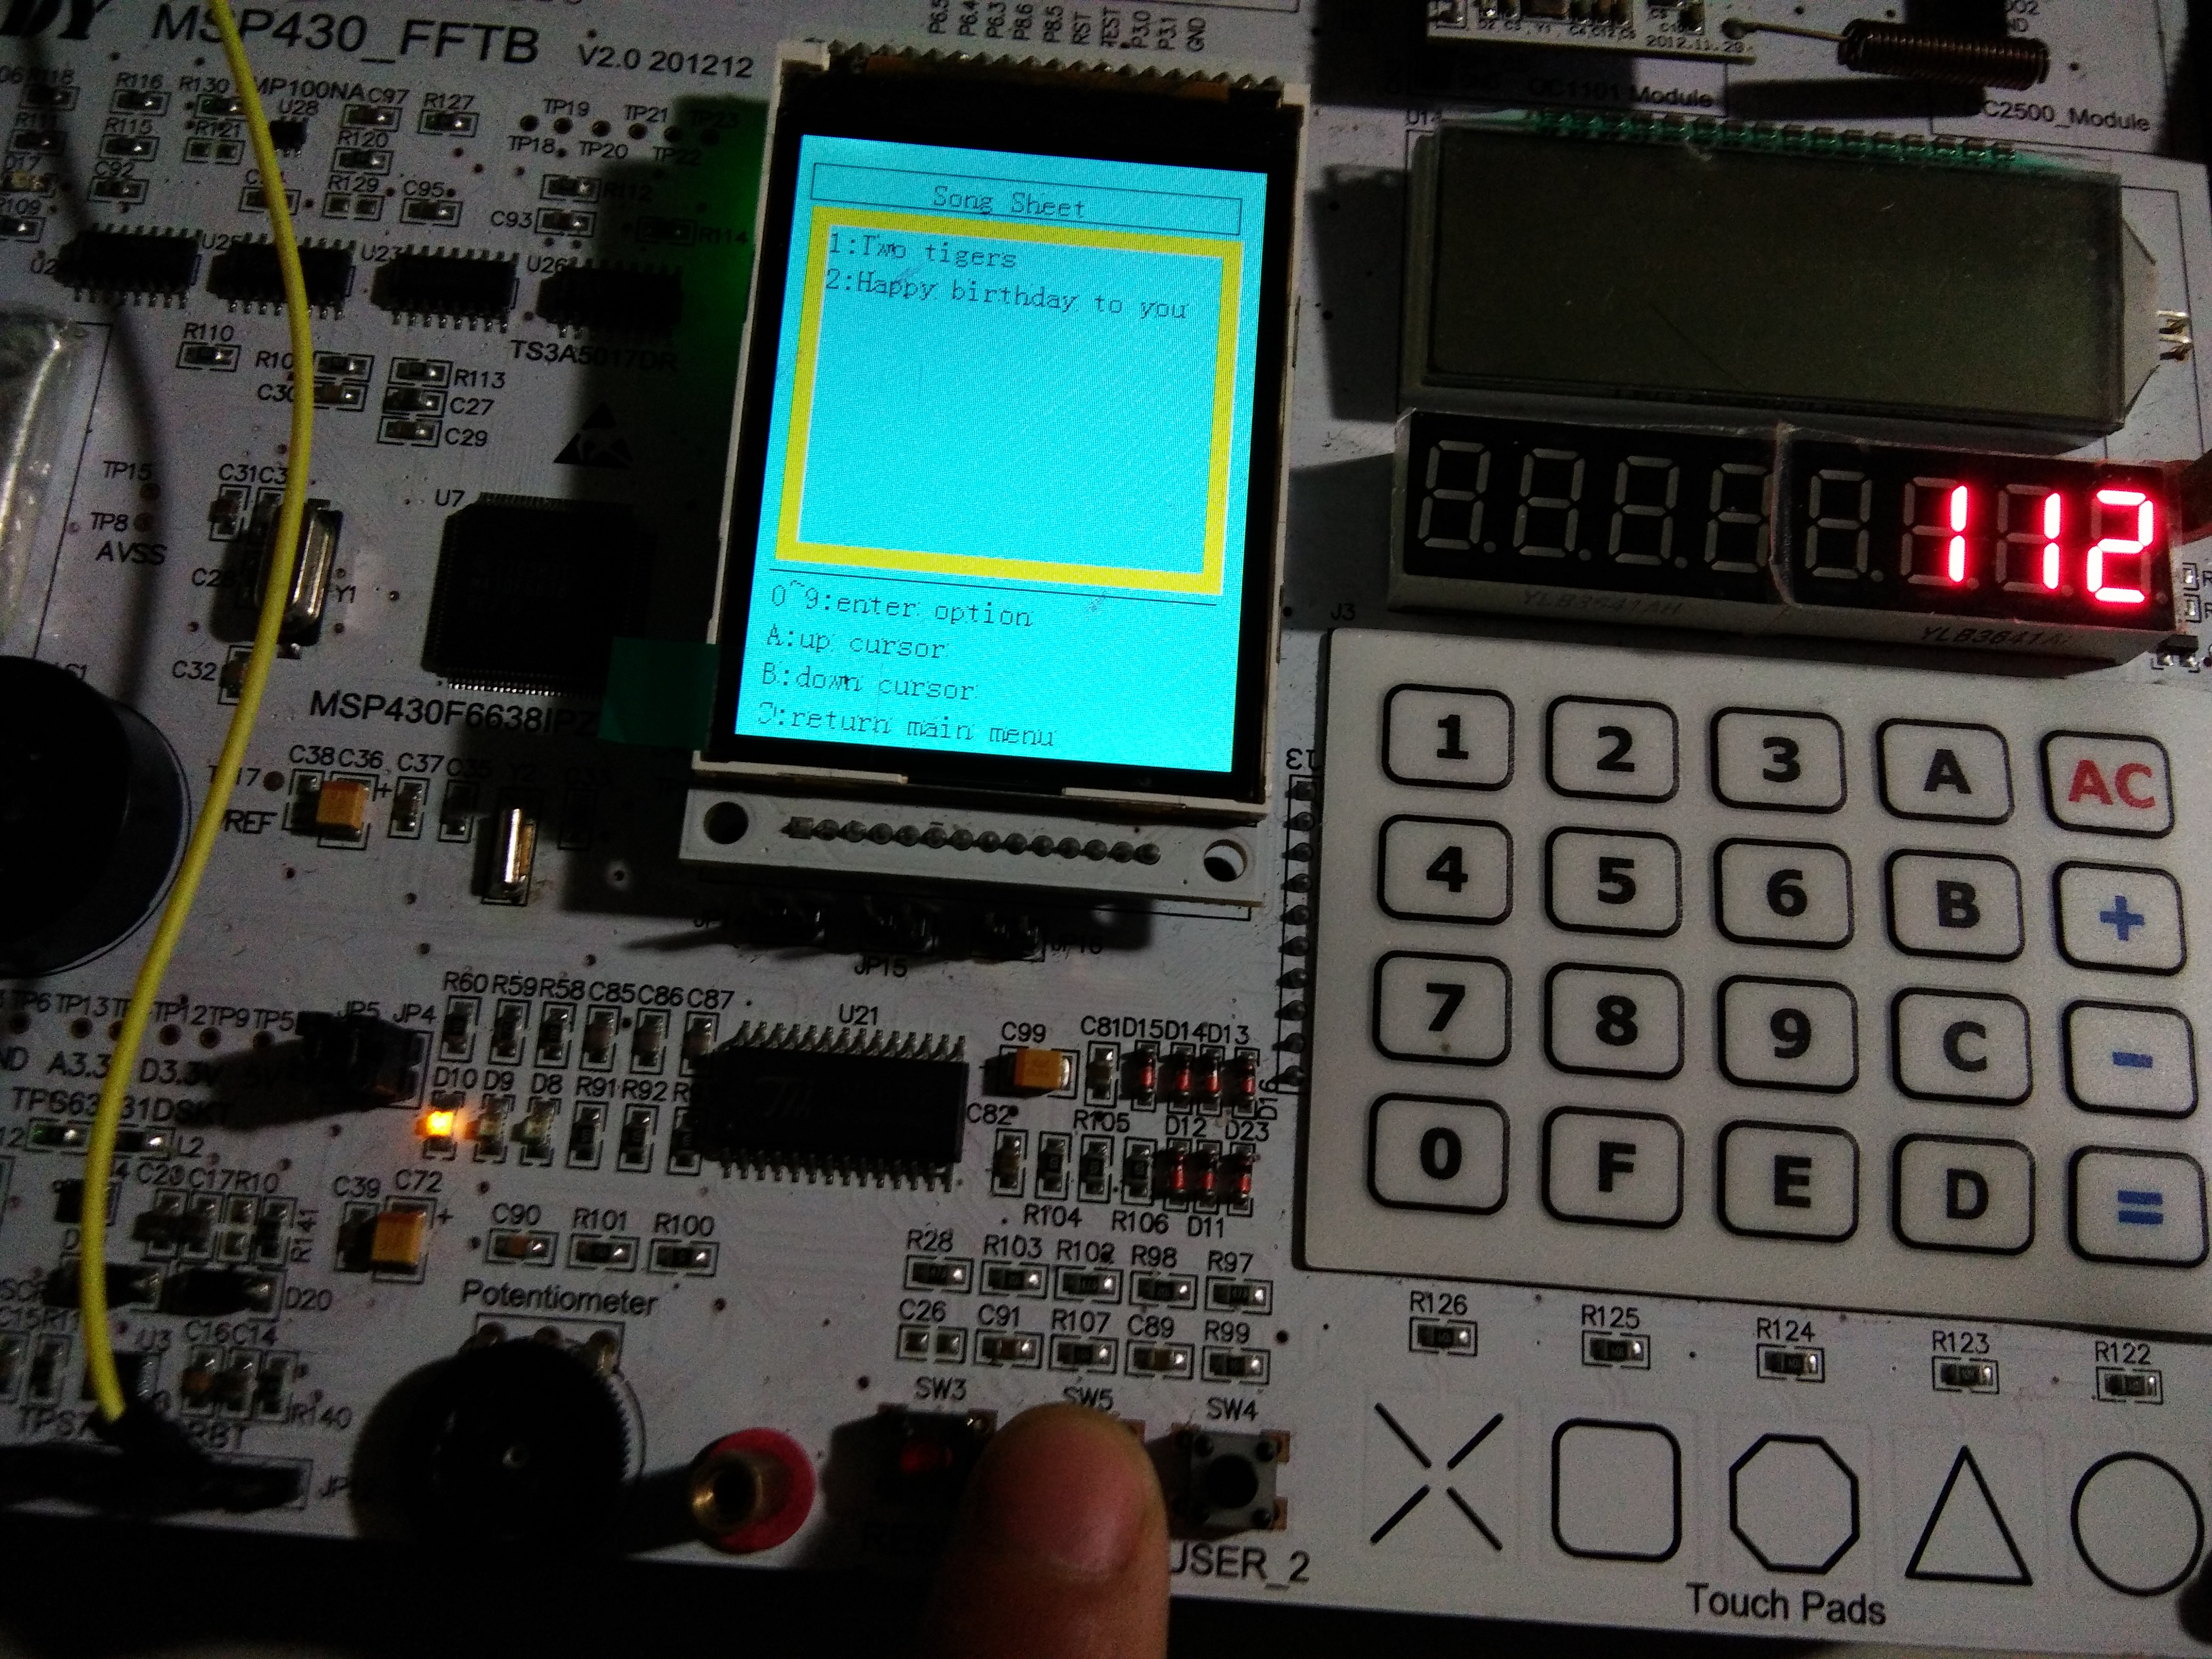
\includegraphics[width=7.5cm]{bitmap/jpg/MusicPlayer5.jpg}
	\end{minipage}
	\begin{minipage}[htbp]{7.5cm}
		\centering
		\caption{按User\_2开关音量}
		\label{MusicPlayer6}
		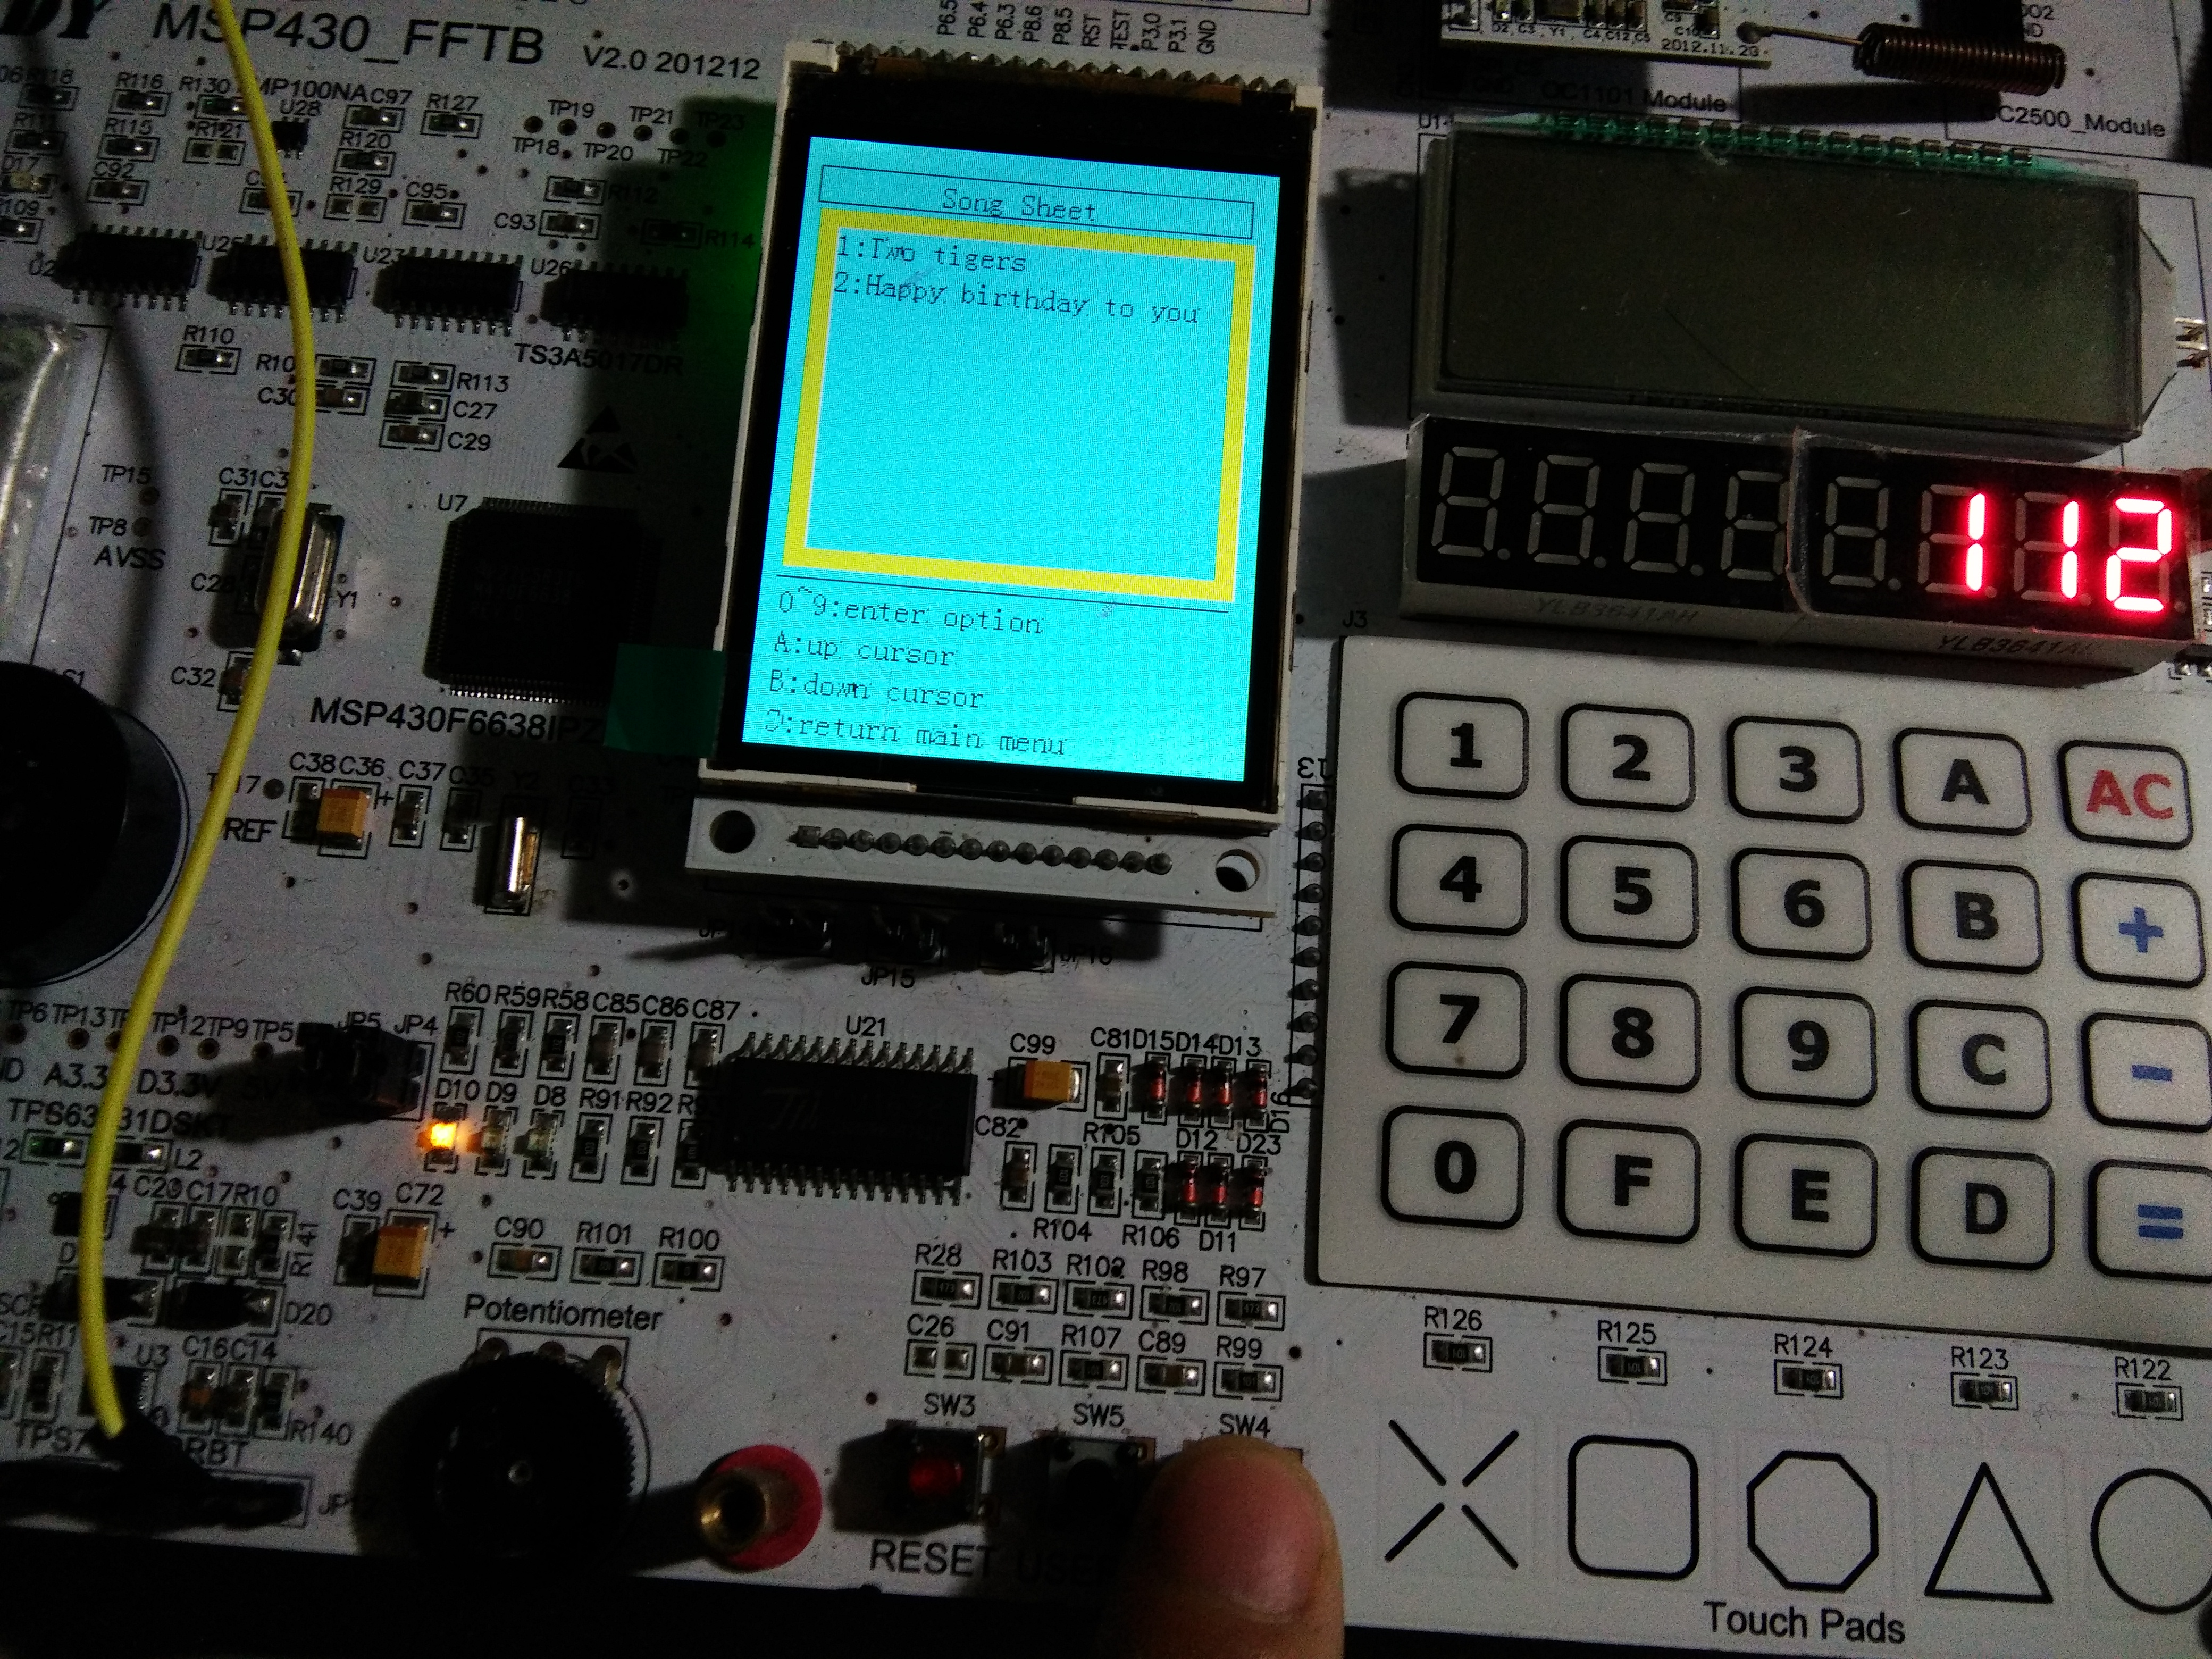
\includegraphics[width=7.5cm]{bitmap/jpg/MusicPlayer6.jpg}
	\end{minipage}
\end{figure}
\begin{figure}[htbp]
	\centering
	\begin{minipage}[htbp]{7.5cm}
		\centering
		\caption{按C返回主界面}
		\label{MusicPlayer7}
		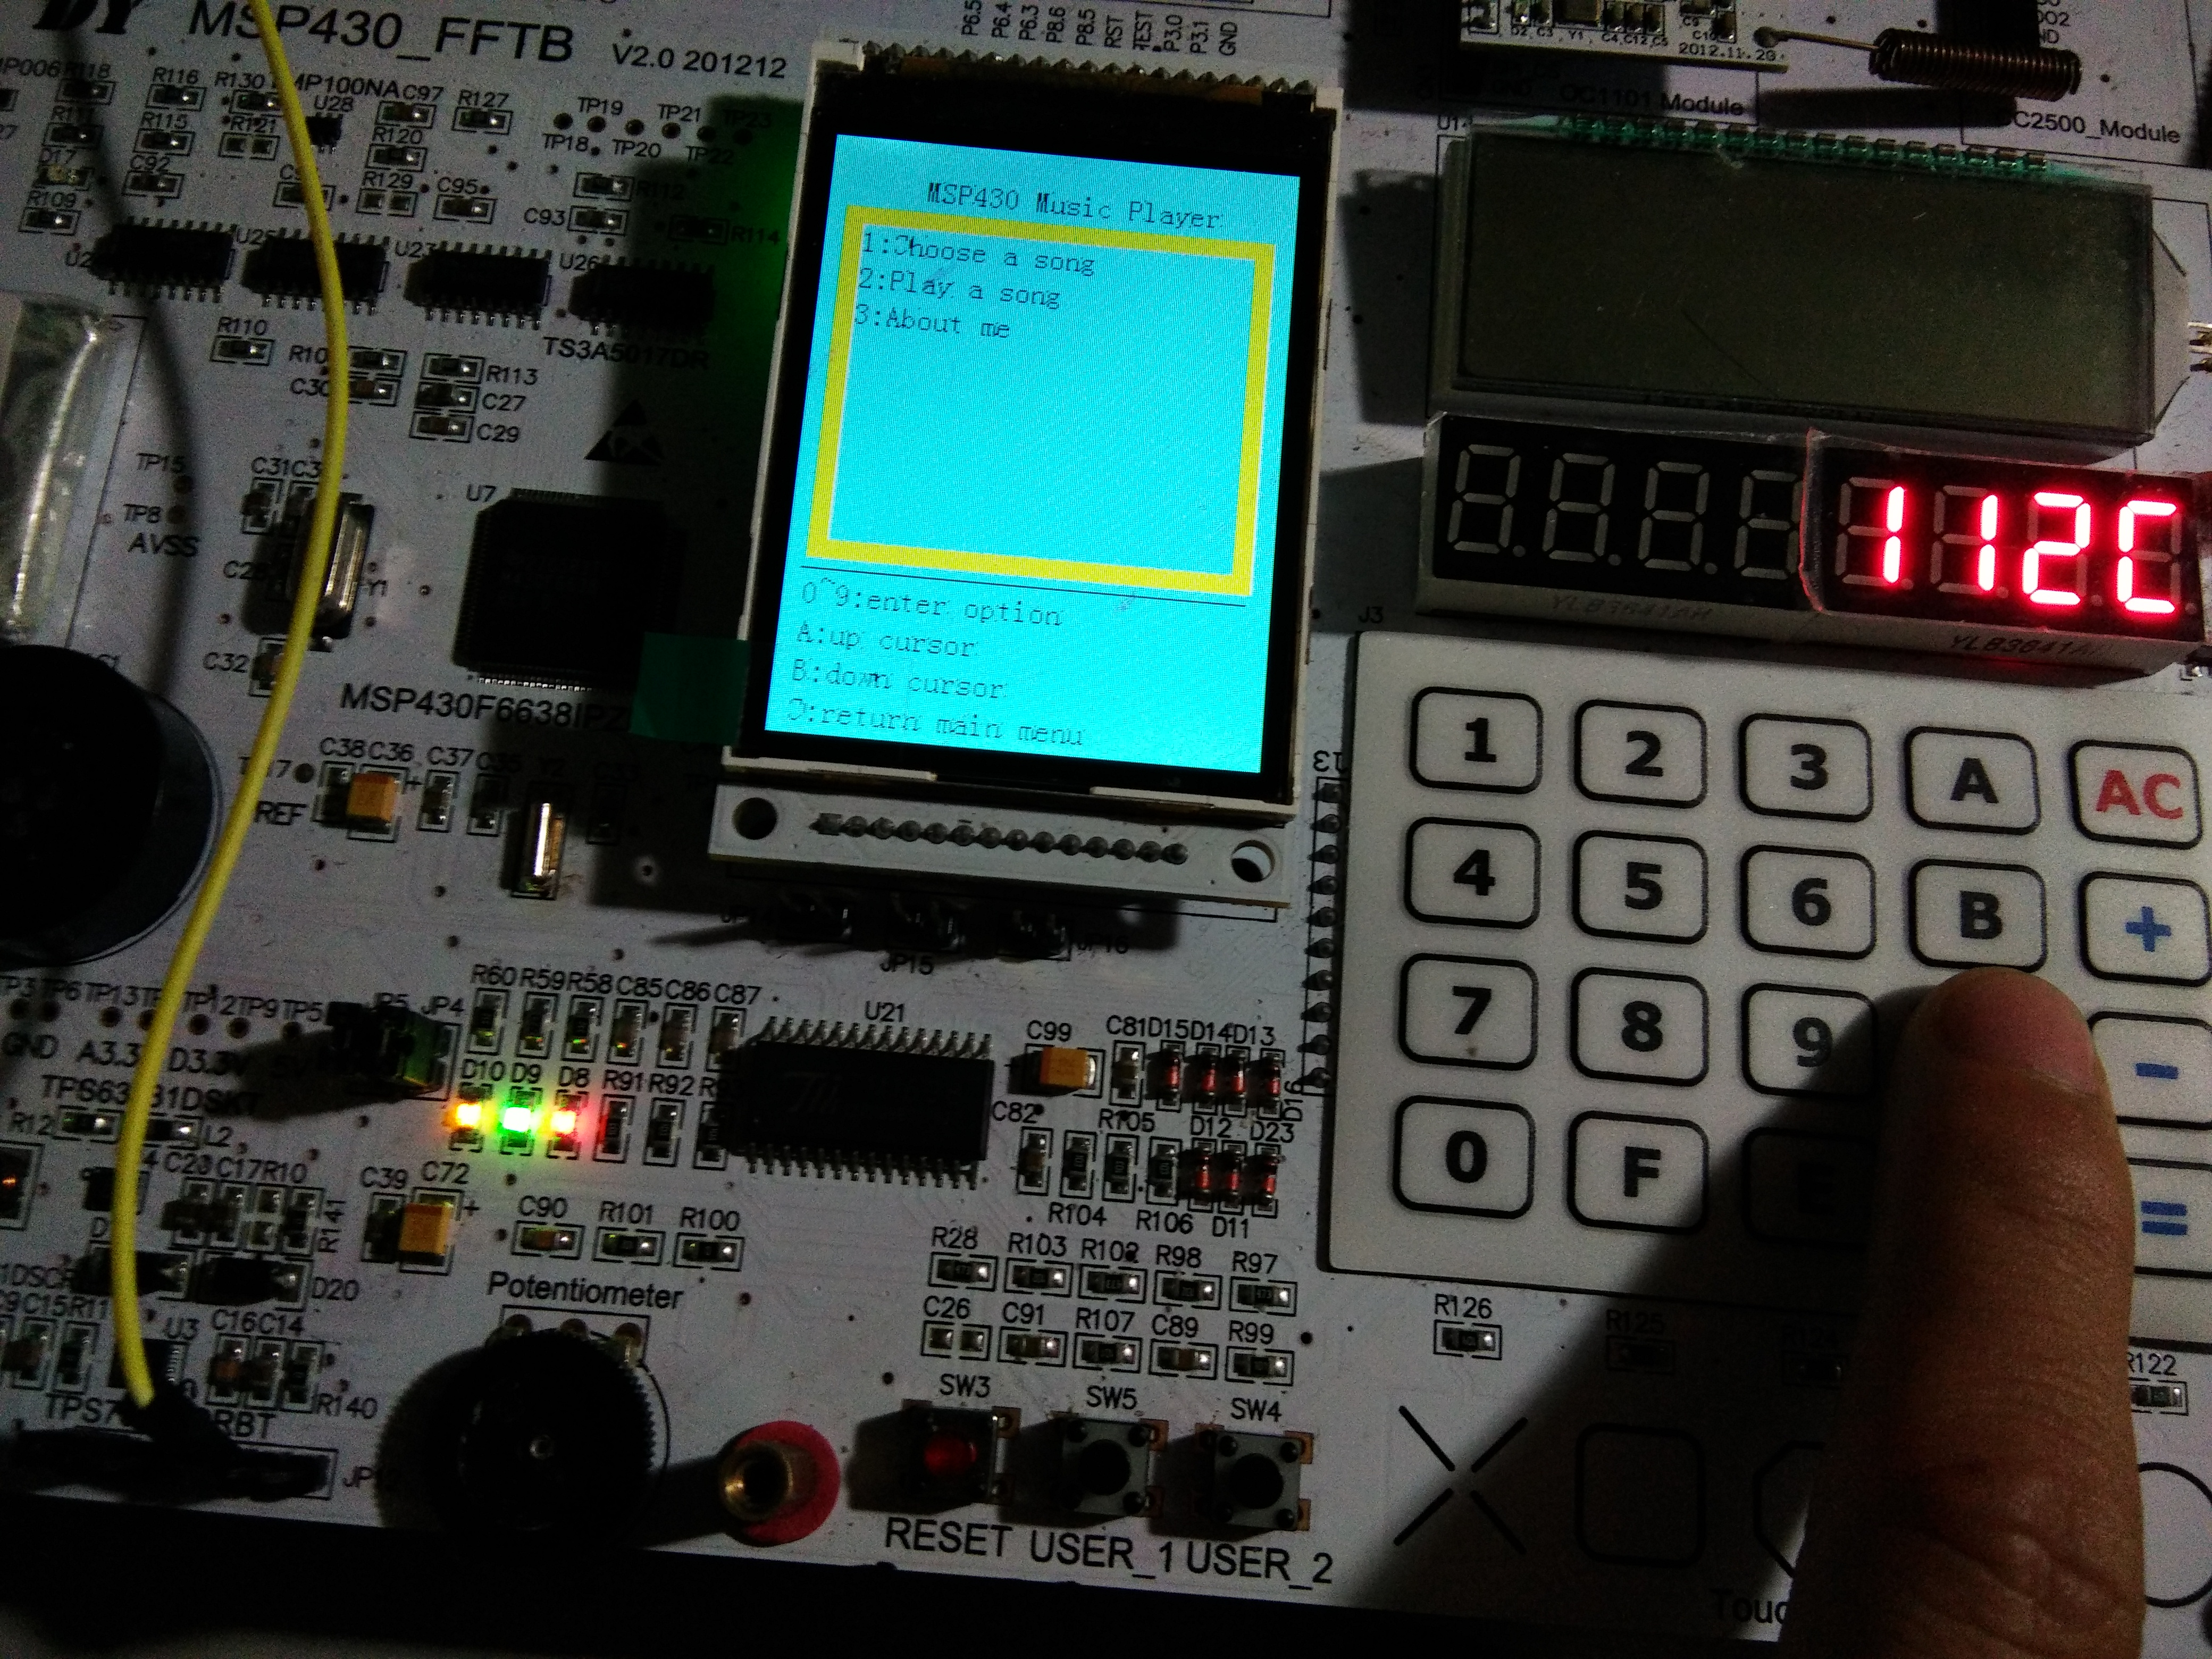
\includegraphics[width=7.5cm]{bitmap/jpg/MusicPlayer7.jpg}
	\end{minipage}
	\begin{minipage}[htbp]{7.5cm}
		\centering
		\caption{按2进入弹奏界面}
		\label{MusicPlayer8}
		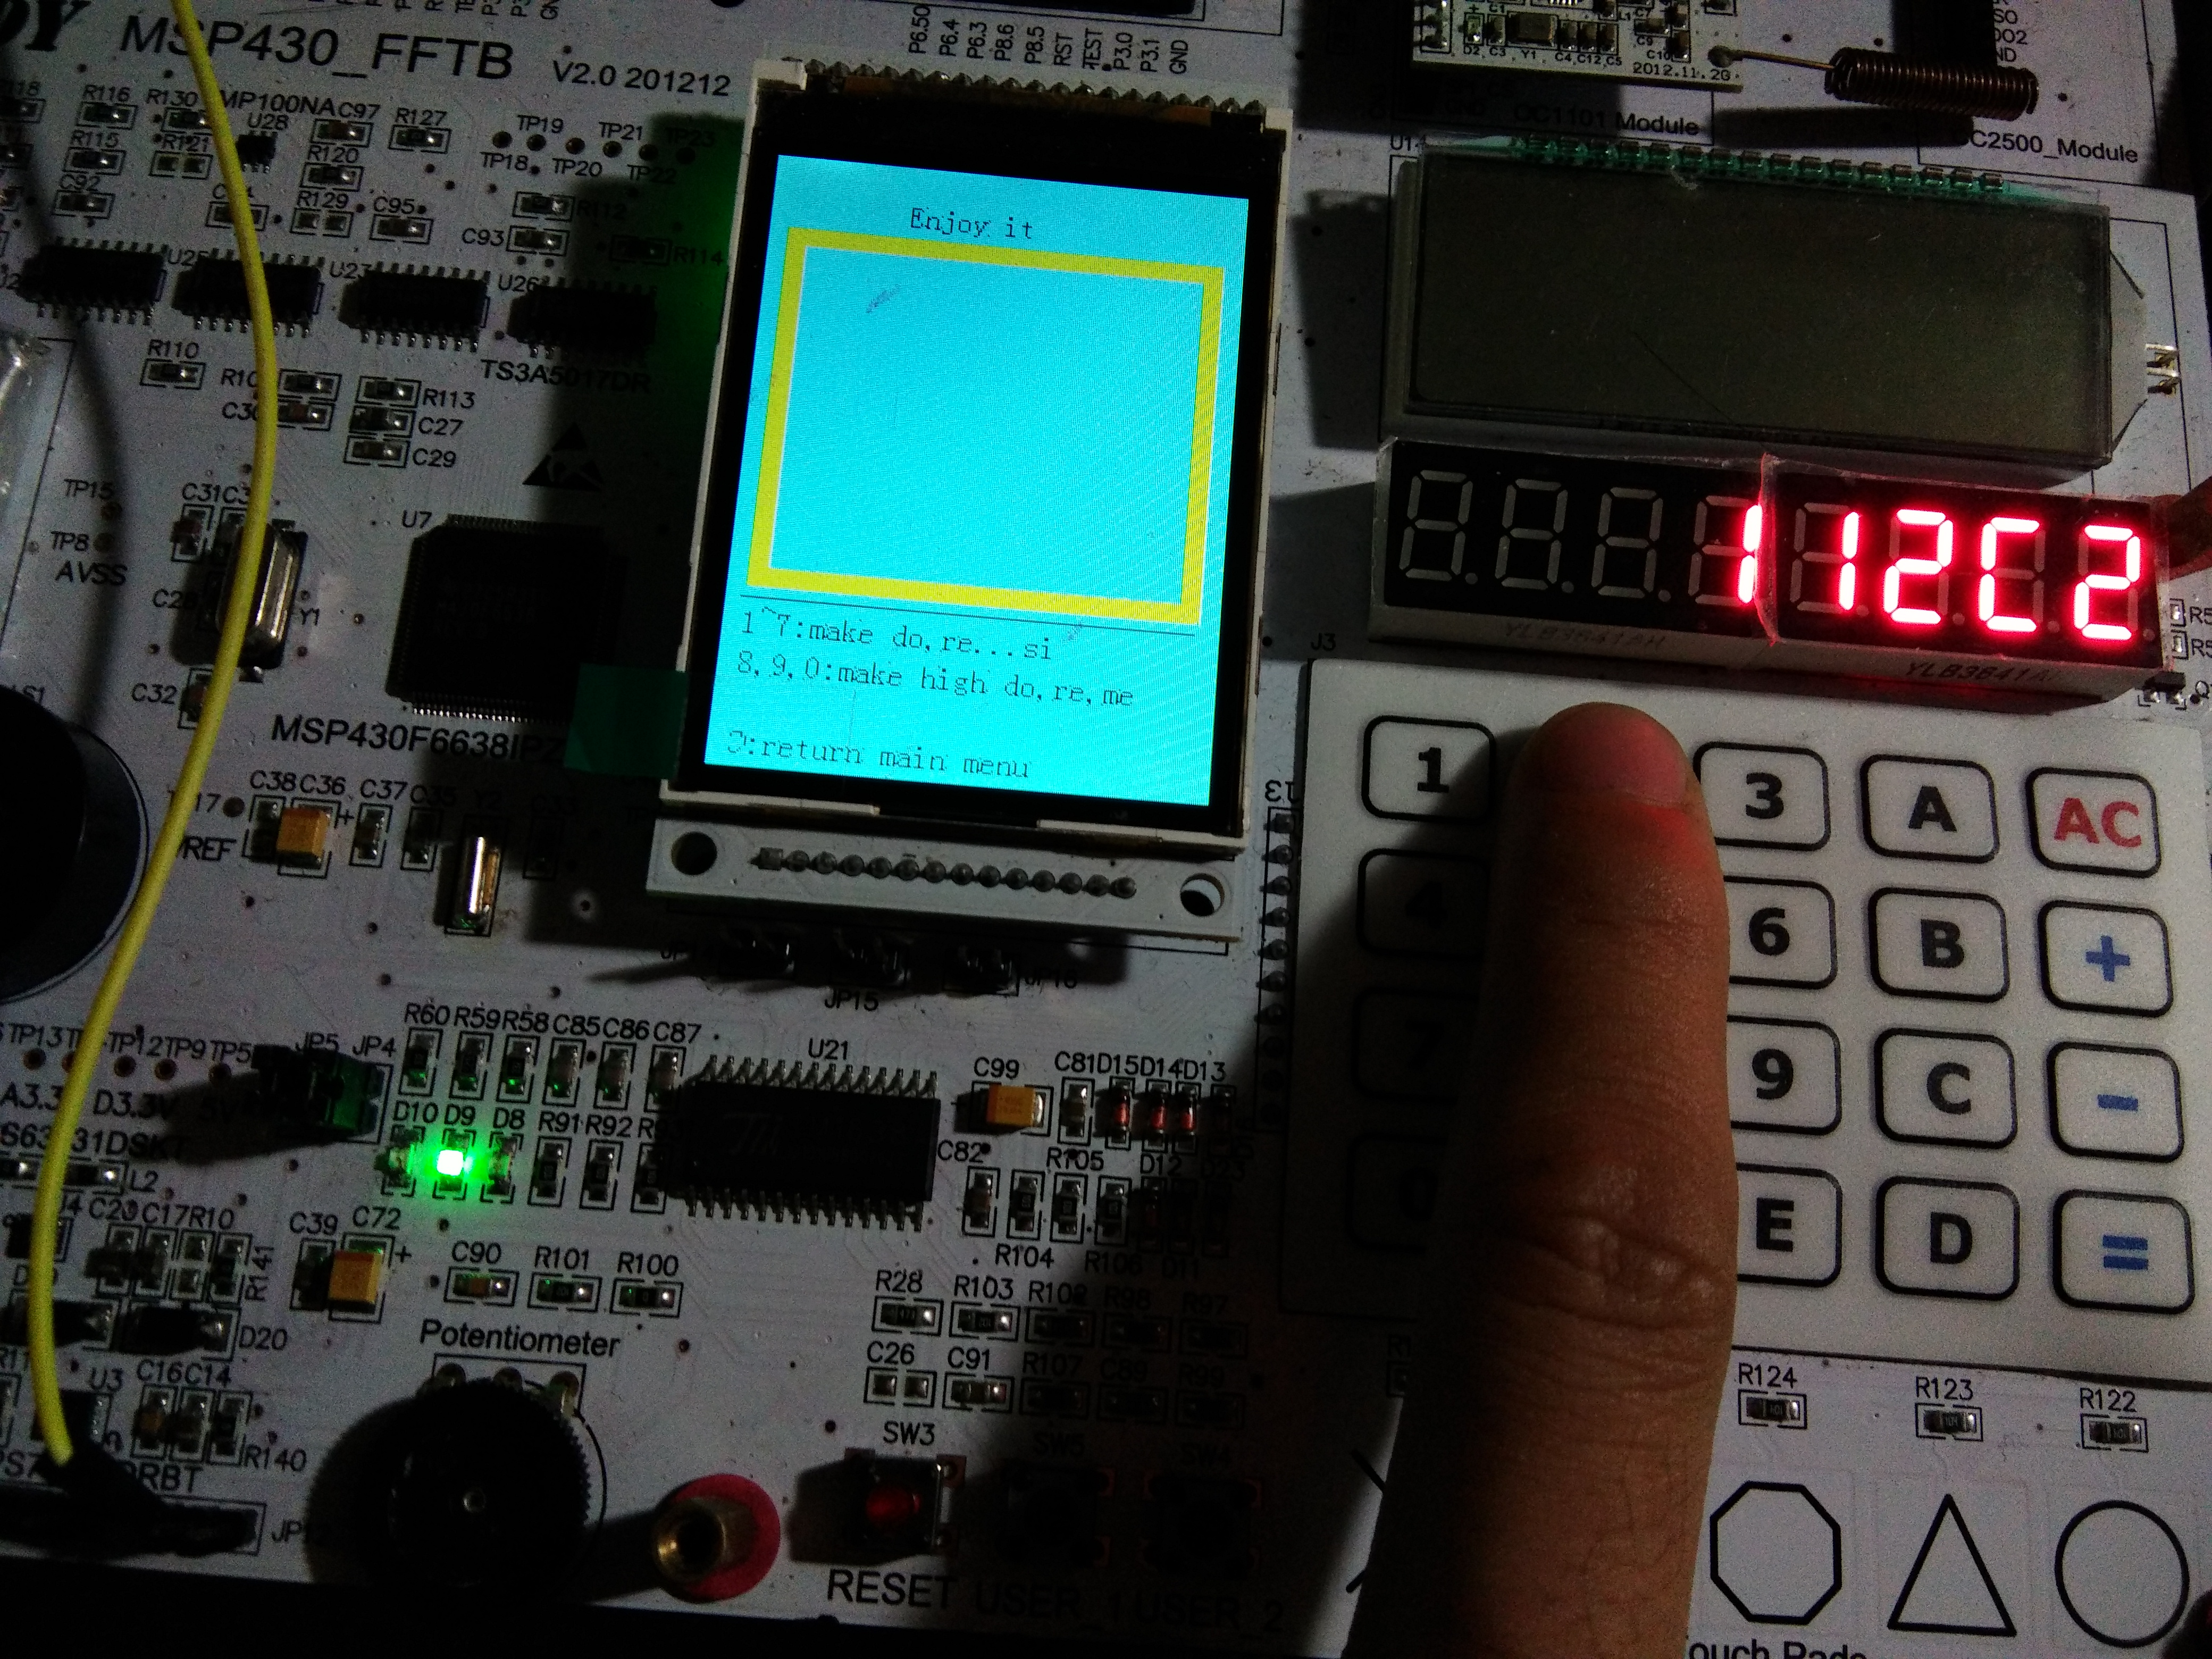
\includegraphics[width=7.5cm]{bitmap/jpg/MusicPlayer8.jpg}
	\end{minipage}
	\begin{minipage}[htbp]{7.5cm}
		\centering
		\caption{按1弹奏do}
		\label{MusicPlayer9}
		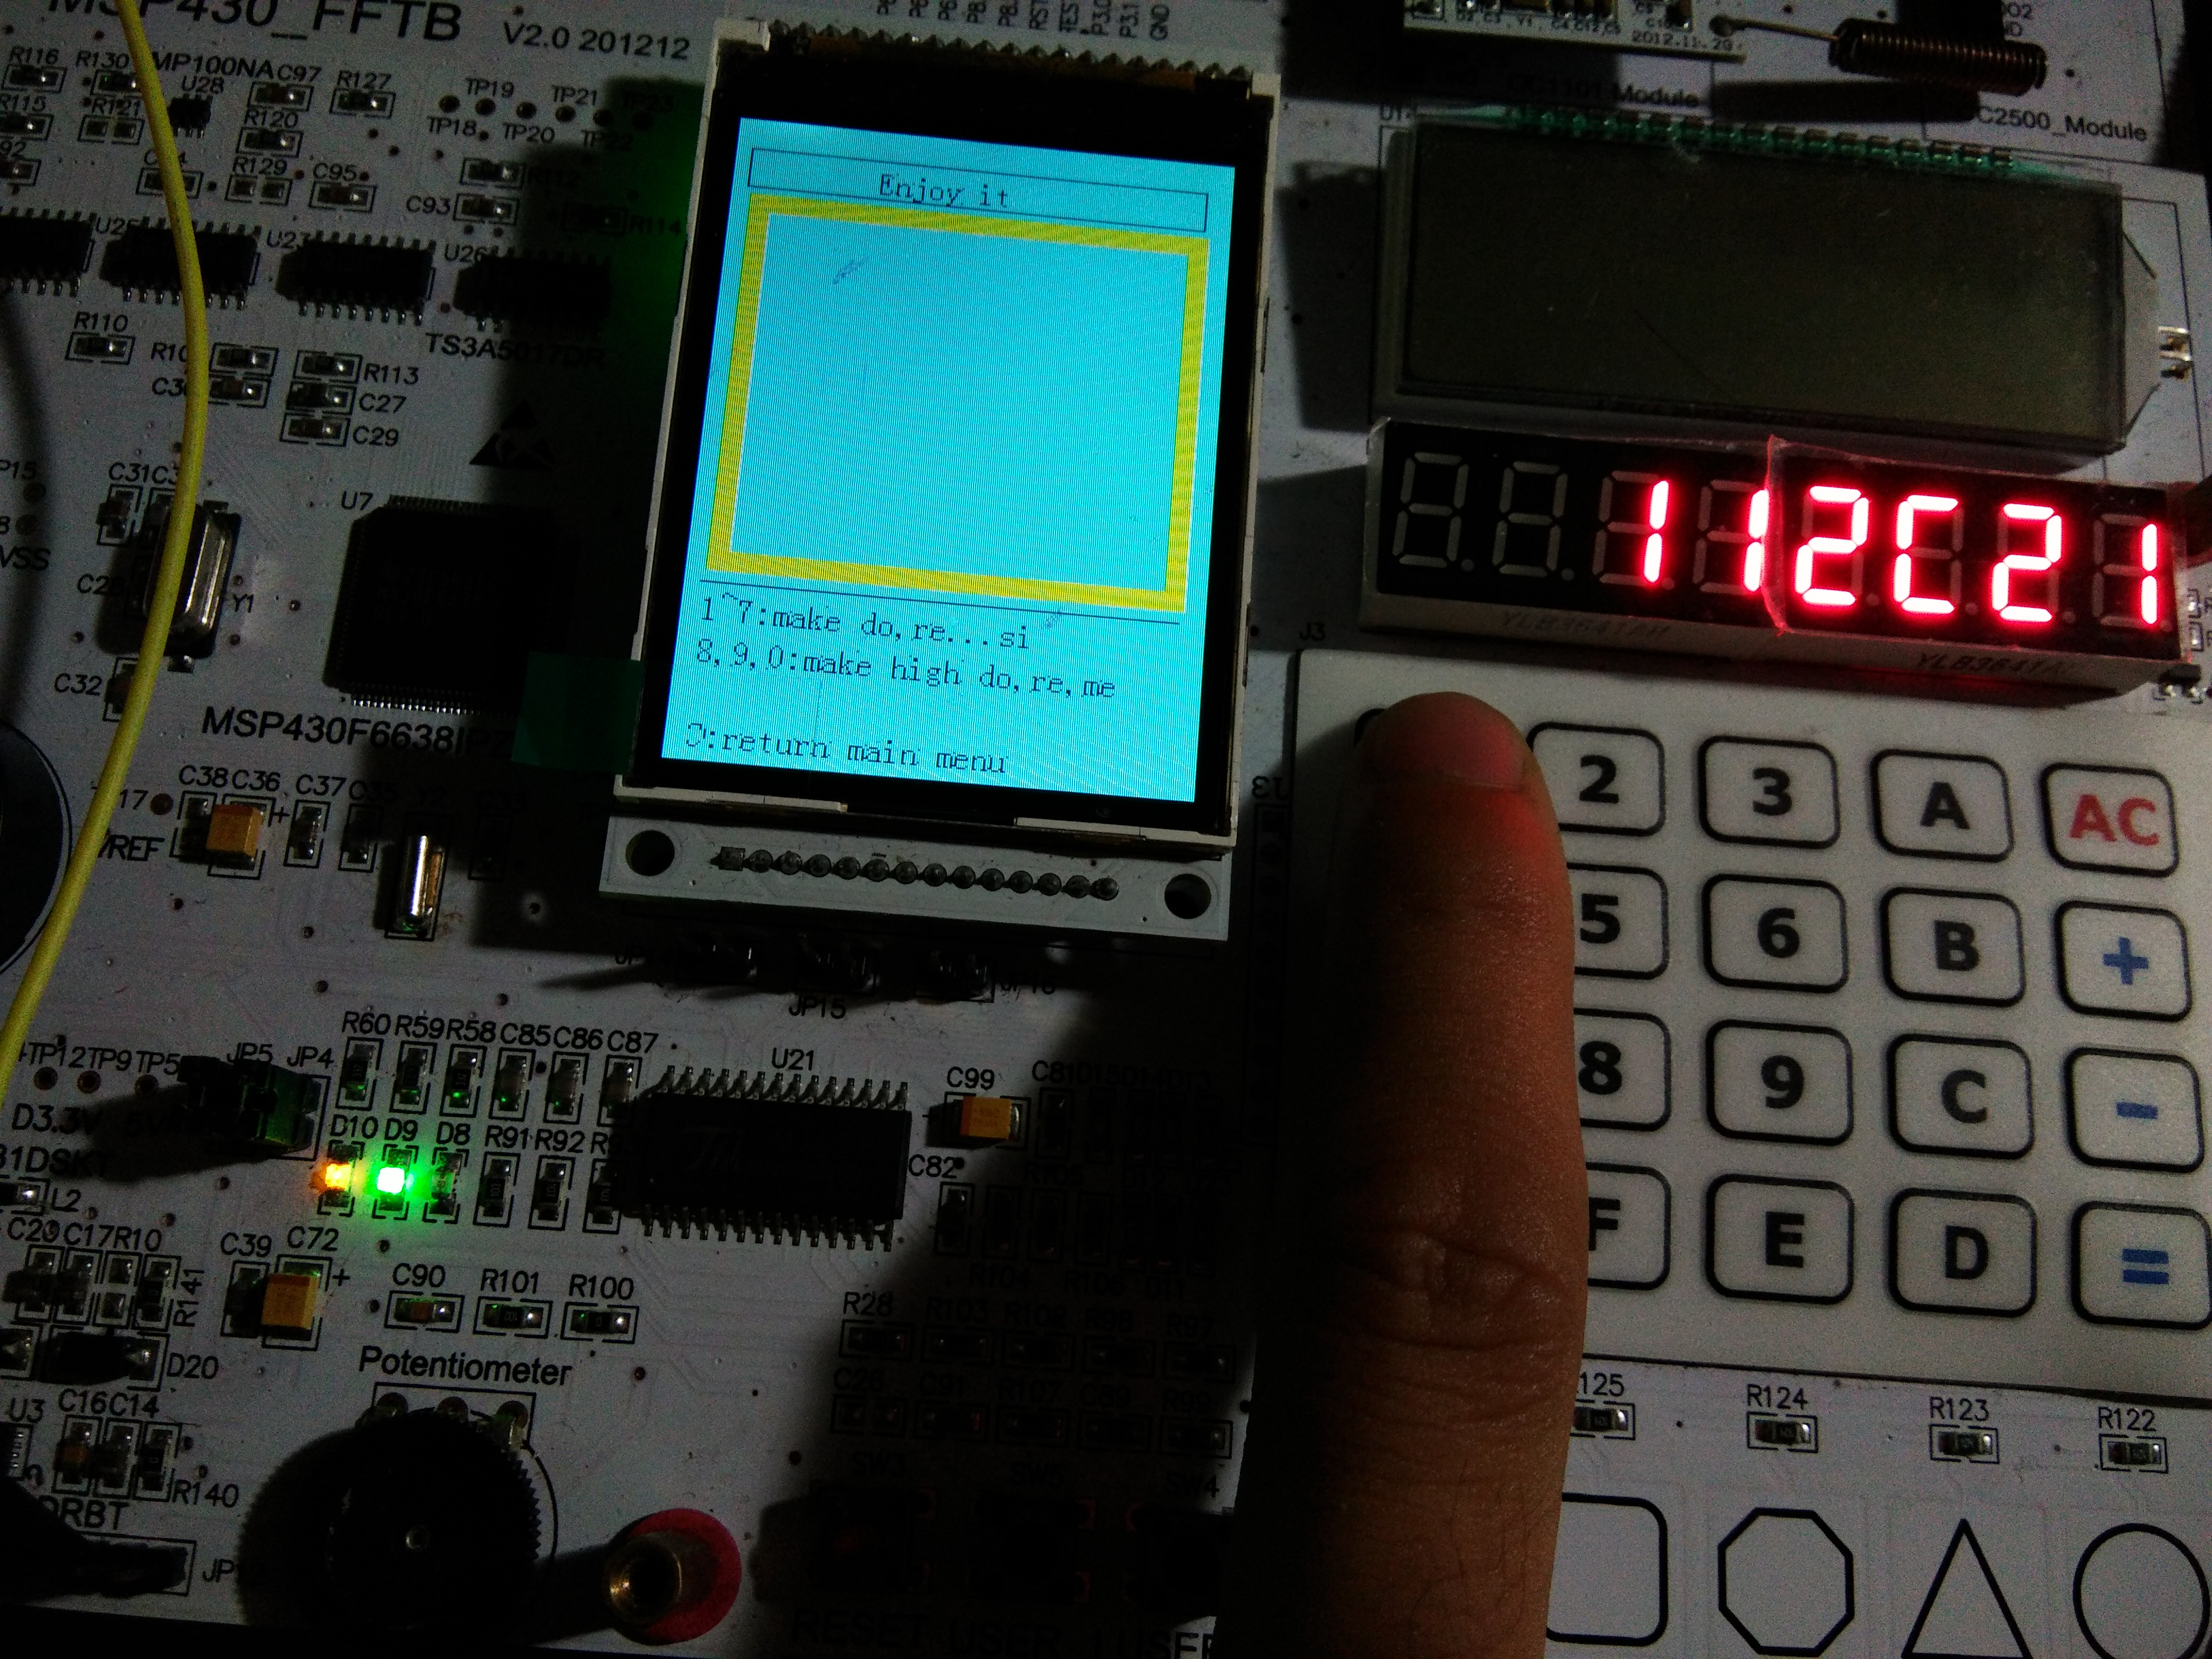
\includegraphics[width=7.5cm]{bitmap/jpg/MusicPlayer9.jpg}
	\end{minipage}
	\begin{minipage}[htbp]{7.5cm}
		\centering
		\caption{按C返回主界面}
		\label{MusicPlayer10}
		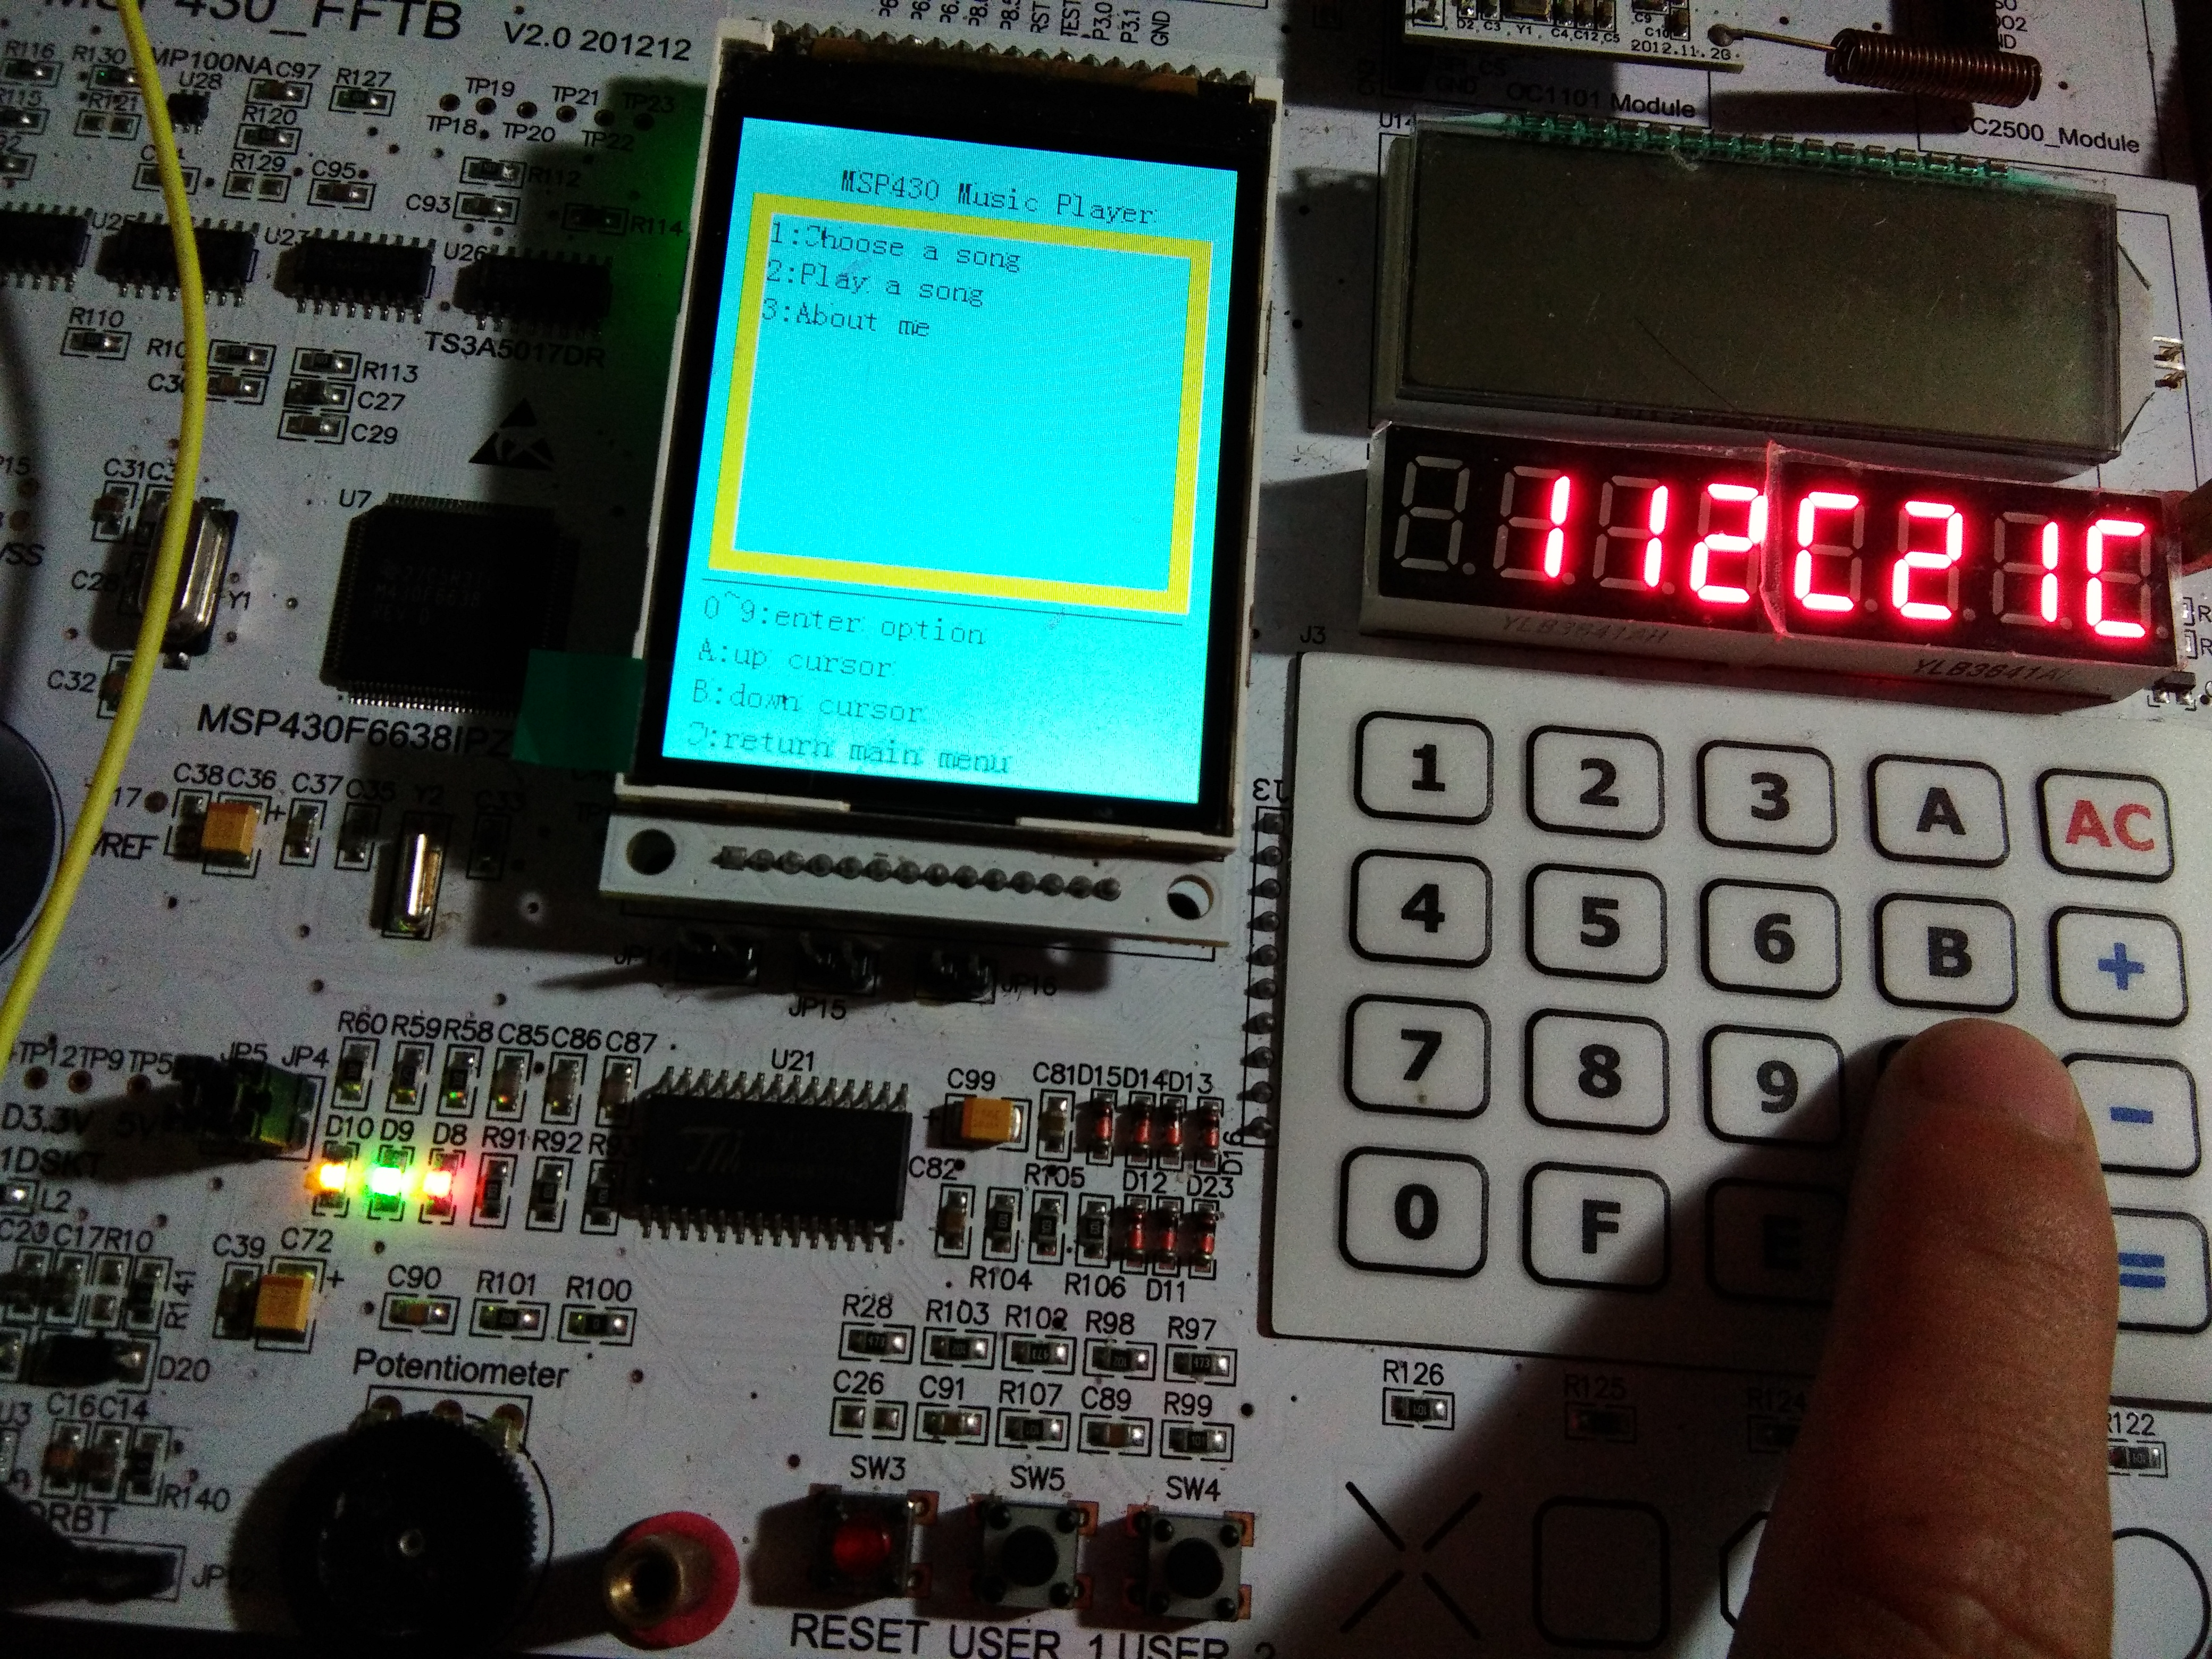
\includegraphics[width=7.5cm]{bitmap/jpg/MusicPlayer10.jpg}
	\end{minipage}
	\begin{minipage}[htbp]{7.5cm}
		\centering
		\caption{按3进入用户信息界面}
		\label{MusicPlayer11}
		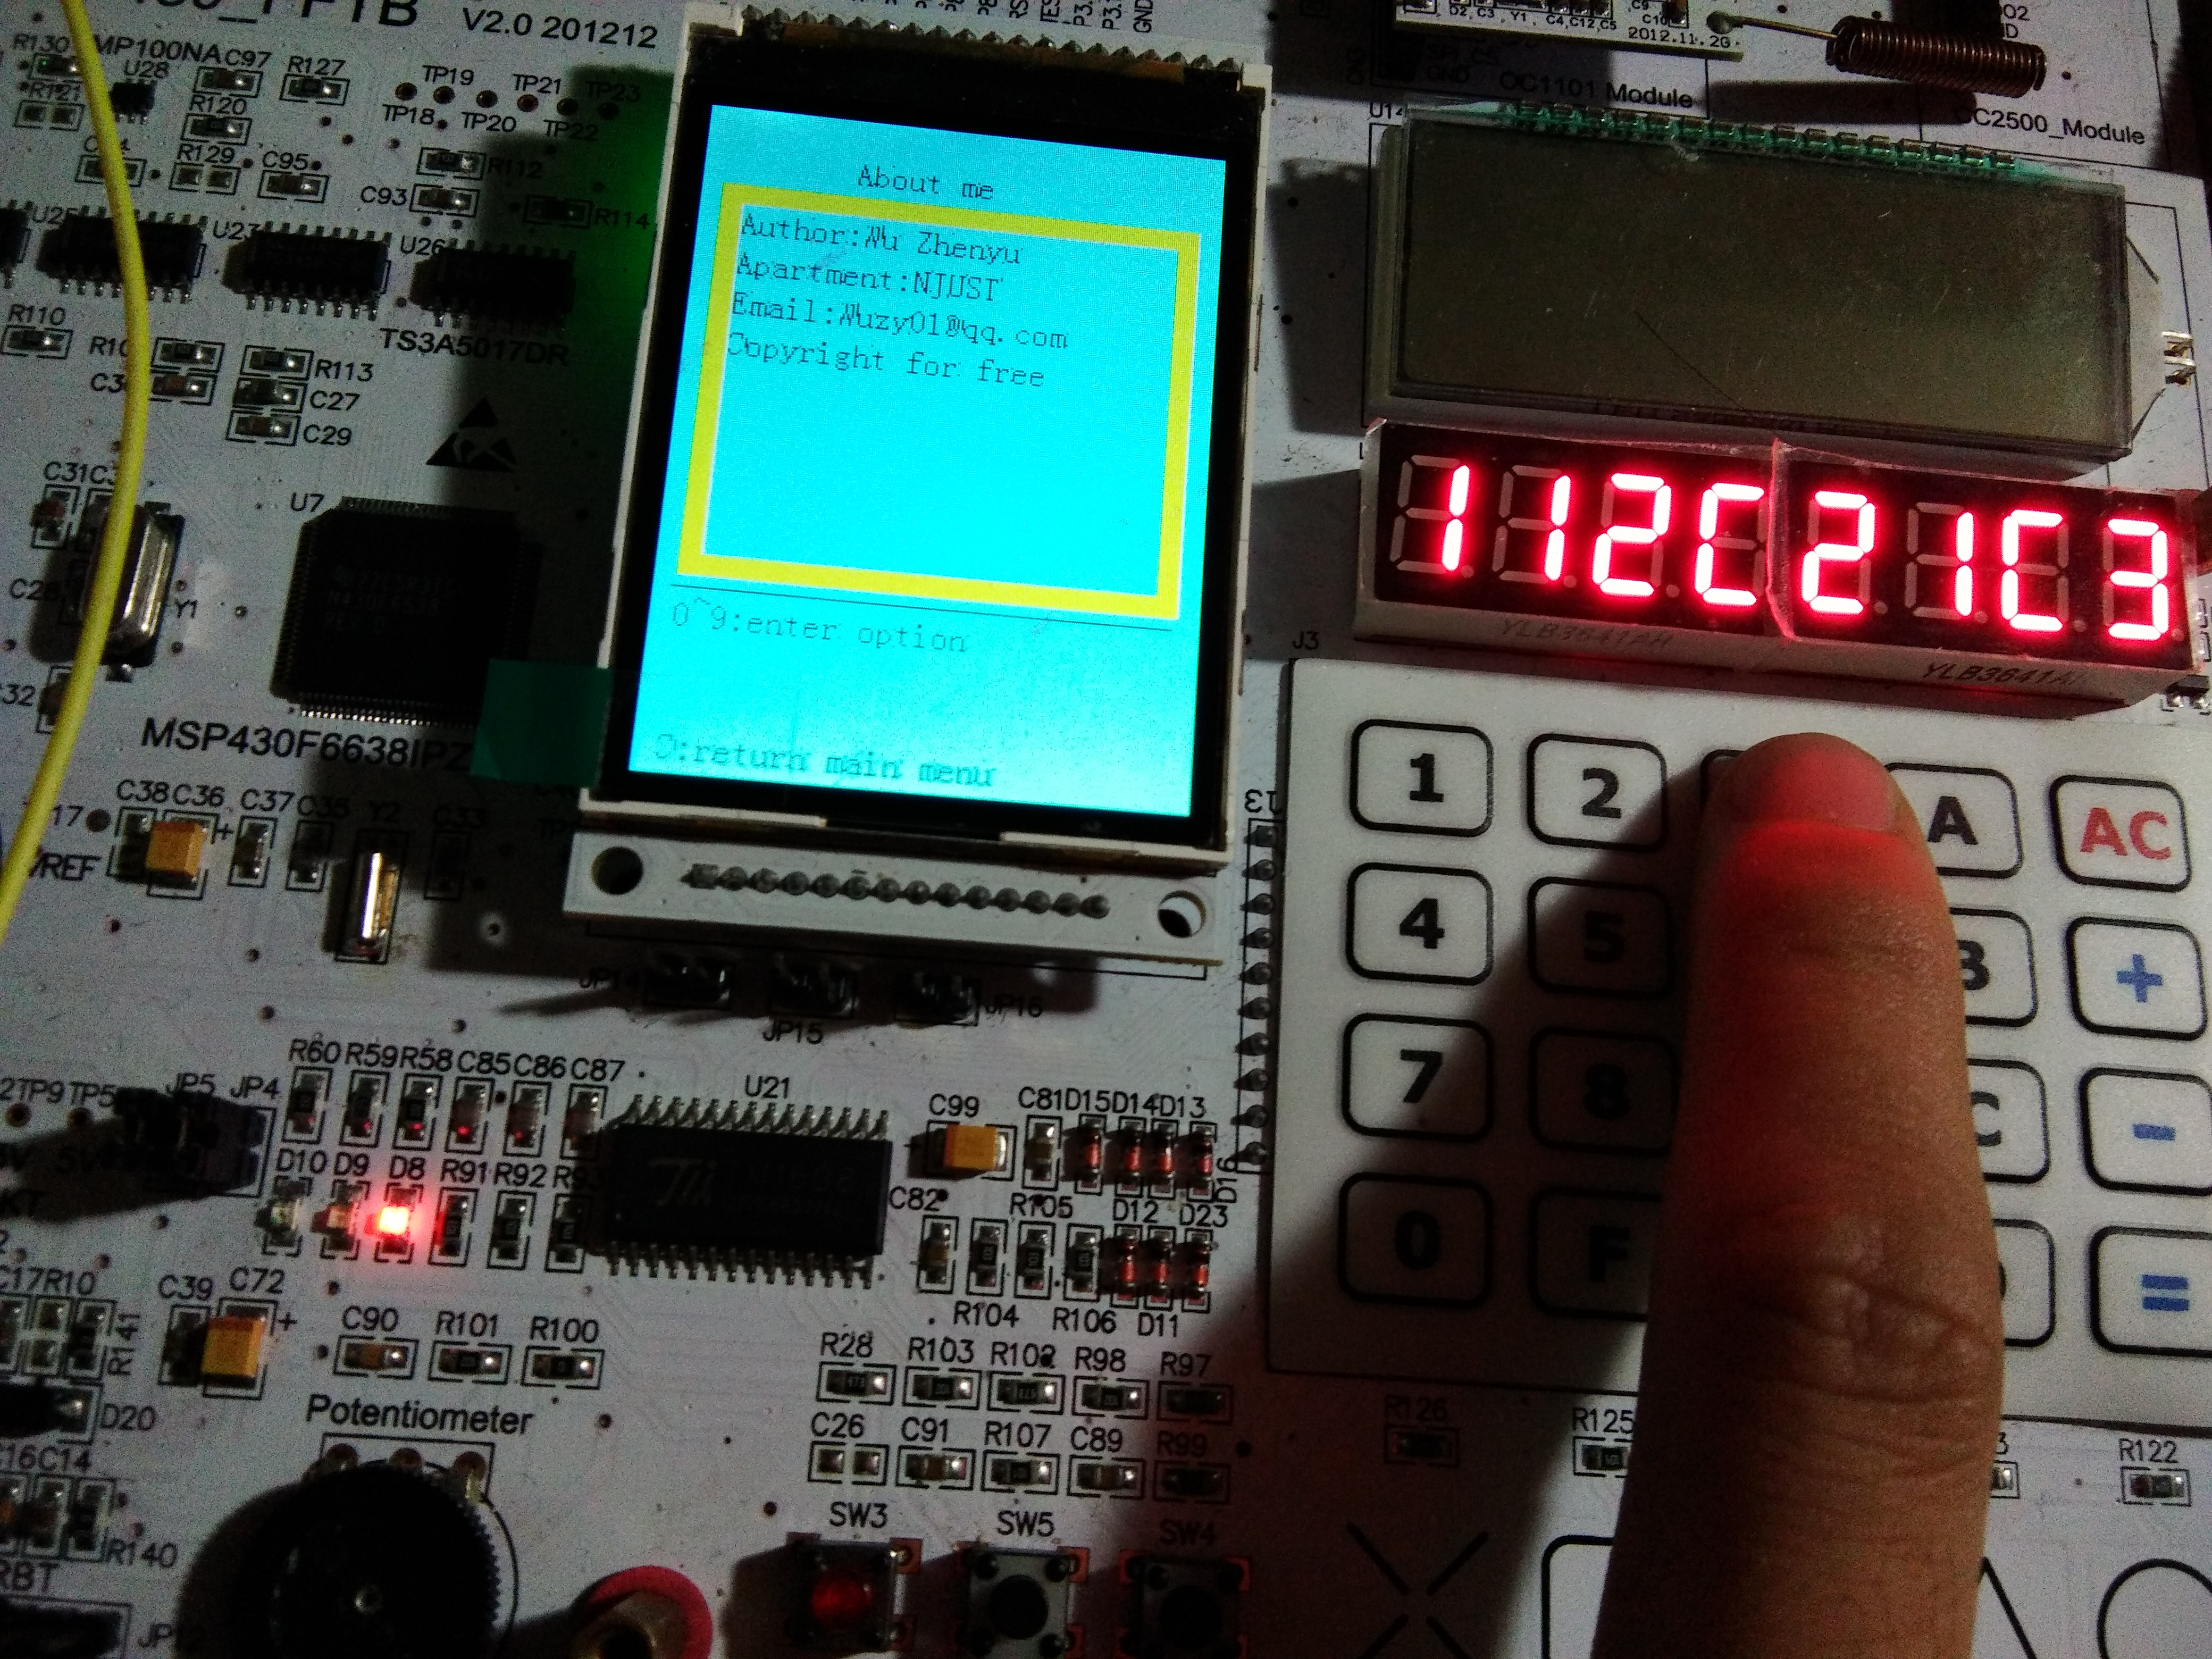
\includegraphics[width=7.5cm]{bitmap/jpg/MusicPlayer11.jpg}
	\end{minipage}
	\begin{minipage}[htbp]{7.5cm}
		\centering
		\caption{按C返回主界面}
		\label{MusicPlayer12}
		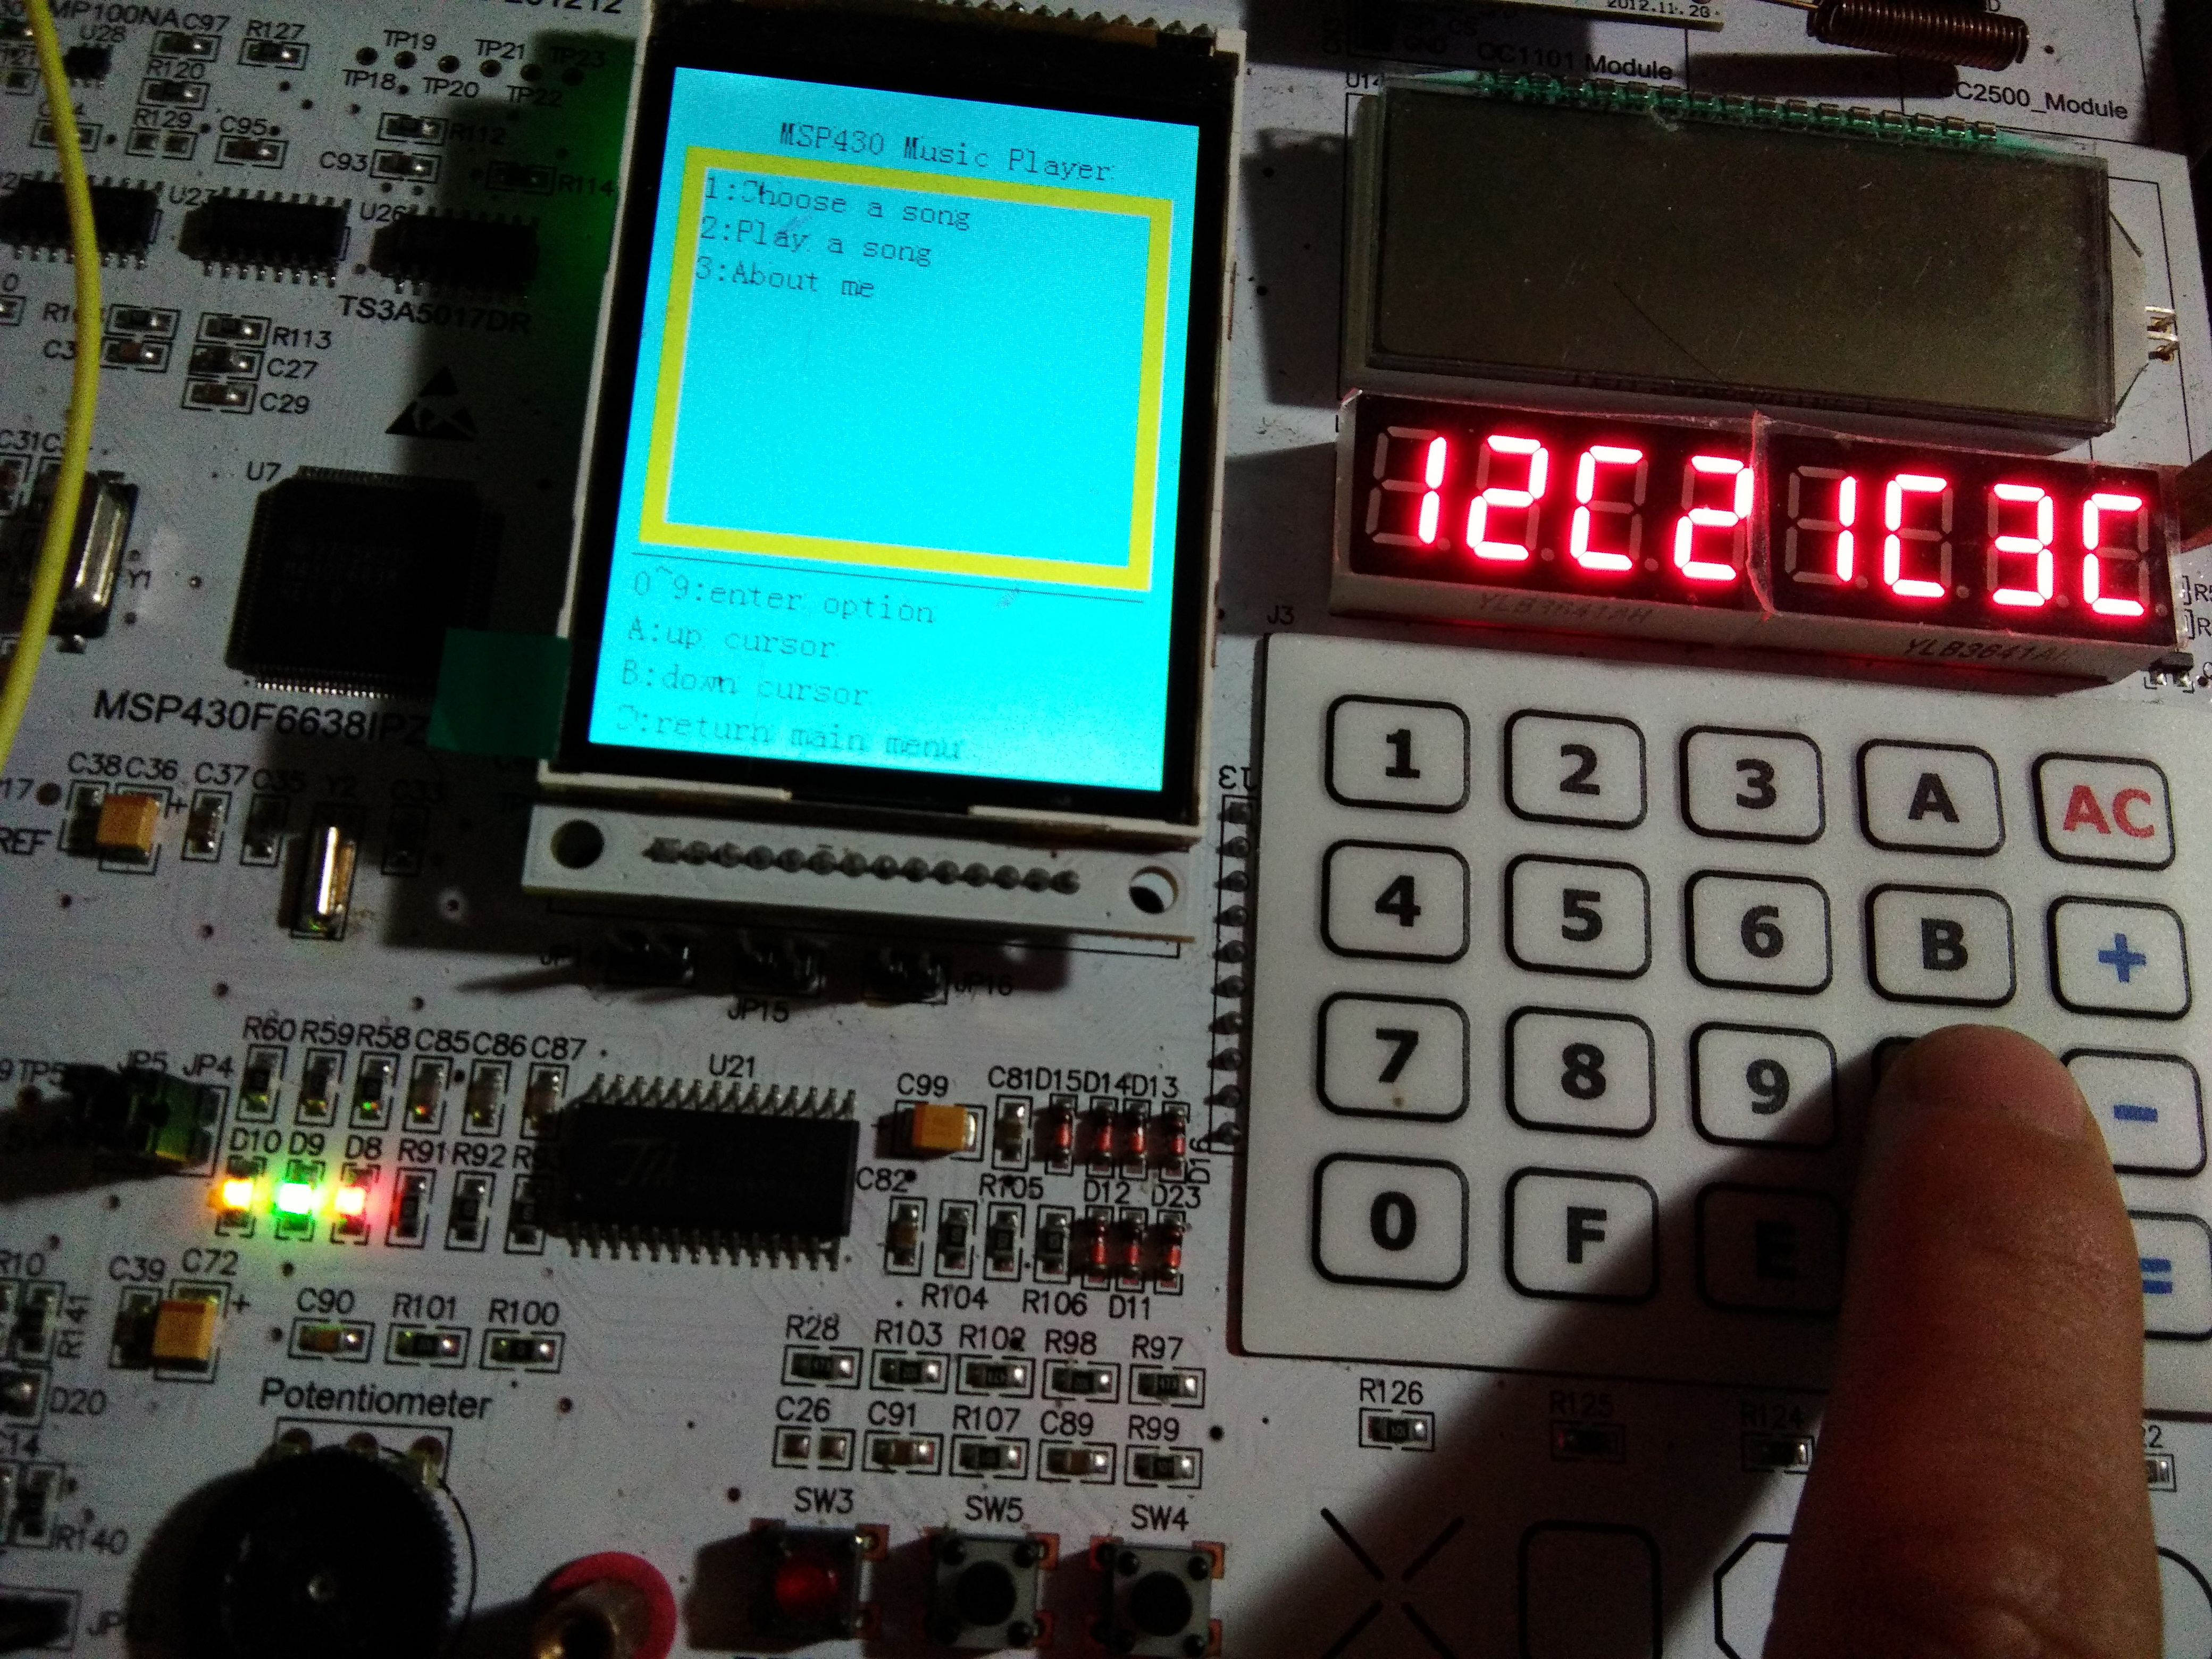
\includegraphics[width=7.5cm]{bitmap/jpg/MusicPlayer12.jpg}
	\end{minipage}
\end{figure}
\begin{figure}[htbp]
	\centering
	\caption{按AC清空历史记录}
	\label{MusicPlayer13}
	\includegraphics[width=8cm]{bitmap/jpg/MusicPlayer13.jpg}
\end{figure}
\newpage
\subsection{遇到的问题与解决方法}
\begin{enumerate}
	\item 最后一个实验也是最难的实验。寄存器寻址做嵌入式开发难度大,调试繁琐,周期长。这最后1个实验总算是可以用库函数做1个真正的软件了。利用MSP430设计一款音乐播放器,俗称随声听。
	\item 首先是库函数的选择。energia和MSPWare、HAL都是TI官方的库,特点如下:
	\begin{table}[htbp]
		\centering
		\caption{MSP430库函数}
		\label{MSP430库函数}
			\begin{longtabu}to\hsize{@{}*4{X[c]}@{}}\toprule
			\diagbox{特点}{库}&energia&MSPWare&HAL\\\midrule
			学习难度&低&中&中\\
			兼容性&AVR的arduino库和STM32的Maple库&无&STM32的HAL库\\
			图形化编程界面&ardublock和KRobot&Grace&HALCoGen\\\bottomrule
			\end{longtabu}
	\end{table}
	\par\indent 3个我都下载了看了一下。在下载MSPWare时费了点功夫,jre安装出错,重装了CCS最新的8.3版本才解决问题。最终使用的还是HAL库,见图\ref{MusicPlayer}。
	\item 主要是6个模块:扬声器、TFT显示屏、独立键盘、LED灯、矩阵键盘及共用tm1638芯片的LCD显示屏。先让每个模块可以独立工作,在一个模块一个模块累加在一起,最后保证所有模块都可以正常工作。遇到的问题主要有的库中寄存器直接赋值而不是或等于某位,这样该模块单独可以正常工作,但联调时就会导致别的模块需要的寄存器的某些位又被清0了。
	\item 至于程序算法倒不是什么难事。以前做过类似的作品。不过即便这样还是花了一段时间才完成。
\end{enumerate}
